\begin{tikzpicture}[scale=.2, anchor=base]
\node[draw=black] (sn0x9a68990W9) at (9, -10) {\begin{tikzpicture}[scale=.2]
\node[circle, scale=0.75, fill] (tid0) at (4.5,0){};
\node[circle, scale=0.75, fill] (tid1) at (2.25,1.5){};
\node[circle, scale=0.75, fill, red] (tid4) at (0.75,3){};

\node[circle, scale=0.75, fill] (tid5) at (2.25,3){};

\node[circle, scale=0.75, fill] (tid6) at (3.75,3){};

\draw[](tid1) -- (tid4);
\draw[](tid1) -- (tid5);
\draw[](tid1) -- (tid6);

\node[circle, scale=0.75, fill] (tid2) at (6,1.5){};
\node[circle, scale=0.75, fill, red] (tid7) at (5.25,3){};

\node[circle, scale=0.75, fill] (tid8) at (6.75,3){};

\draw[](tid2) -- (tid7);
\draw[](tid2) -- (tid8);

\node[circle, scale=0.75, fill] (tid3) at (8.25,1.5){};
\node[circle, scale=0.75, fill] (tid9) at (8.25,3){};

\draw[](tid3) -- (tid9);

\draw[](tid0) -- (tid1);
\draw[](tid0) -- (tid2);
\draw[](tid0) -- (tid3);

\end{tikzpicture}
};
\node[draw=black] (sn0x9a68730W9) at (9, -20) {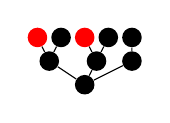
\begin{tikzpicture}[scale=.2]
\node[circle, scale=0.75, fill] (tid0) at (3.75,0){};
\node[circle, scale=0.75, fill] (tid1) at (1.5,1.5){};
\node[circle, scale=0.75, fill, red] (tid4) at (0.75,3){};

\node[circle, scale=0.75, fill] (tid5) at (2.25,3){};

\draw[](tid1) -- (tid4);
\draw[](tid1) -- (tid5);

\node[circle, scale=0.75, fill] (tid2) at (4.5,1.5){};
\node[circle, scale=0.75, fill, red] (tid6) at (3.75,3){};

\node[circle, scale=0.75, fill] (tid7) at (5.25,3){};

\draw[](tid2) -- (tid6);
\draw[](tid2) -- (tid7);

\node[circle, scale=0.75, fill] (tid3) at (6.75,1.5){};
\node[circle, scale=0.75, fill] (tid8) at (6.75,3){};

\draw[](tid3) -- (tid8);

\draw[](tid0) -- (tid1);
\draw[](tid0) -- (tid2);
\draw[](tid0) -- (tid3);

\end{tikzpicture}
};
\node[draw=black] (sn0x9a696c8W9) at (9, -30) {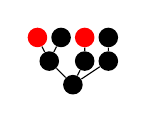
\begin{tikzpicture}[scale=.2]
\node[circle, scale=0.75, fill] (tid0) at (3,0){};
\node[circle, scale=0.75, fill] (tid1) at (1.5,1.5){};
\node[circle, scale=0.75, fill, red] (tid4) at (0.75,3){};

\node[circle, scale=0.75, fill] (tid5) at (2.25,3){};

\draw[](tid1) -- (tid4);
\draw[](tid1) -- (tid5);

\node[circle, scale=0.75, fill] (tid2) at (3.75,1.5){};
\node[circle, scale=0.75, fill, red] (tid6) at (3.75,3){};

\draw[](tid2) -- (tid6);

\node[circle, scale=0.75, fill] (tid3) at (5.25,1.5){};
\node[circle, scale=0.75, fill] (tid7) at (5.25,3){};

\draw[](tid3) -- (tid7);

\draw[](tid0) -- (tid1);
\draw[](tid0) -- (tid2);
\draw[](tid0) -- (tid3);

\end{tikzpicture}
};
\node[draw=black] (sn0x9a6cfd8W9) at (9, -40) {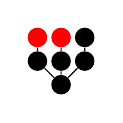
\begin{tikzpicture}[scale=.2]
\node[circle, scale=0.75, fill] (tid0) at (2.25,0){};
\node[circle, scale=0.75, fill] (tid1) at (0.75,1.5){};
\node[circle, scale=0.75, fill, red] (tid4) at (0.75,3){};

\draw[](tid1) -- (tid4);

\node[circle, scale=0.75, fill] (tid2) at (2.25,1.5){};
\node[circle, scale=0.75, fill, red] (tid5) at (2.25,3){};

\draw[](tid2) -- (tid5);

\node[circle, scale=0.75, fill] (tid3) at (3.75,1.5){};
\node[circle, scale=0.75, fill] (tid6) at (3.75,3){};

\draw[](tid3) -- (tid6);

\draw[](tid0) -- (tid1);
\draw[](tid0) -- (tid2);
\draw[](tid0) -- (tid3);

\end{tikzpicture}
};
\node[draw=black] (sn0x9a6d750W9) at (9, -50) {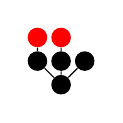
\begin{tikzpicture}[scale=.2]
\node[circle, scale=0.75, fill] (tid0) at (2.25,0){};
\node[circle, scale=0.75, fill] (tid1) at (0.75,1.5){};
\node[circle, scale=0.75, fill, red] (tid4) at (0.75,3){};

\draw[](tid1) -- (tid4);

\node[circle, scale=0.75, fill] (tid2) at (2.25,1.5){};
\node[circle, scale=0.75, fill, red] (tid5) at (2.25,3){};

\draw[](tid2) -- (tid5);

\node[circle, scale=0.75, fill] (tid3) at (3.75,1.5){};

\draw[](tid0) -- (tid1);
\draw[](tid0) -- (tid2);
\draw[](tid0) -- (tid3);

\end{tikzpicture}
};
\node[draw=black] (sn0x9a6da10W9) at (9, -60) {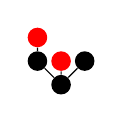
\begin{tikzpicture}[scale=.2]
\node[circle, scale=0.75, fill] (tid0) at (2.25,0){};
\node[circle, scale=0.75, fill] (tid1) at (0.75,1.5){};
\node[circle, scale=0.75, fill, red] (tid4) at (0.75,3){};

\draw[](tid1) -- (tid4);

\node[circle, scale=0.75, fill, red] (tid2) at (2.25,1.5){};

\node[circle, scale=0.75, fill] (tid3) at (3.75,1.5){};

\draw[](tid0) -- (tid1);
\draw[](tid0) -- (tid2);
\draw[](tid0) -- (tid3);

\end{tikzpicture}
};
\node[draw=black] (sn0x9a6d990W9) at (9, -70) {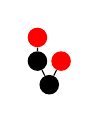
\begin{tikzpicture}[scale=.2]
\node[circle, scale=0.75, fill] (tid0) at (1.5,0){};
\node[circle, scale=0.75, fill] (tid1) at (0.75,1.5){};
\node[circle, scale=0.75, fill, red] (tid3) at (0.75,3){};

\draw[](tid1) -- (tid3);

\node[circle, scale=0.75, fill, red] (tid2) at (2.25,1.5){};

\draw[](tid0) -- (tid1);
\draw[](tid0) -- (tid2);

\end{tikzpicture}
};
\node[draw=black] (sn0x9a6dd40W9) at (9, -80) {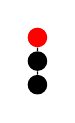
\begin{tikzpicture}[scale=.2]
\node[circle, scale=0.75, fill] (tid0) at (0.75,0){};
\node[circle, scale=0.75, fill] (tid1) at (0.75,1.5){};
\node[circle, scale=0.75, fill, red] (tid2) at (0.75,3){};

\draw[](tid1) -- (tid2);

\draw[](tid0) -- (tid1);

\end{tikzpicture}
};
\node[draw=black] (sn0x9a6e148W9) at (9, -90) {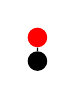
\begin{tikzpicture}[scale=.2]
\node[circle, scale=0.75, fill] (tid0) at (0.75,0){};
\node[circle, scale=0.75, fill, red] (tid1) at (0.75,1.5){};

\draw[](tid0) -- (tid1);

\end{tikzpicture}
};
\node[draw=black] (sn0x9a6e1b0W9) at (9, -100) {
\begin{tikzpicture}[scale=.2]
\node[circle, scale=0.75, fill] (tid0) at (0.75,0){};

\end{tikzpicture}
};
\draw (sn0x9a6e148W9.south) -- (sn0x9a6e1b0W9.north);
\draw (sn0x9a6dd40W9.south) -- (sn0x9a6e148W9.north);
\node[draw=black] (sn0x9a6dff8W18) at (18, -80) {
\begin{tikzpicture}[scale=.2]
\node[circle, scale=0.75, fill] (tid0) at (1.5,0){};
\node[circle, scale=0.75, fill, red] (tid1) at (0.75,1.5){};

\node[circle, scale=0.75, fill, red] (tid2) at (2.25,1.5){};

\draw[](tid0) -- (tid1);
\draw[](tid0) -- (tid2);

\end{tikzpicture}
};
\draw (sn0x9a6dff8W18.south) -- (sn0x9a6e148W9.north);
\draw (sn0x9a6d990W9.south) -- (sn0x9a6dd40W9.north);
\draw (sn0x9a6d990W9.south) -- (sn0x9a6dff8W18.north);
\node[draw=black] (sn0x9a6dcd8W18) at (18, -70) {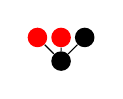
\begin{tikzpicture}[scale=.2]
\node[circle, scale=0.75, fill] (tid0) at (2.25,0){};
\node[circle, scale=0.75, fill, red] (tid1) at (0.75,1.5){};

\node[circle, scale=0.75, fill, red] (tid2) at (2.25,1.5){};

\node[circle, scale=0.75, fill] (tid3) at (3.75,1.5){};

\draw[](tid0) -- (tid1);
\draw[](tid0) -- (tid2);
\draw[](tid0) -- (tid3);

\end{tikzpicture}
};
\draw (sn0x9a6dcd8W18.south) -- (sn0x9a6dff8W18.north);
\draw (sn0x9a6da10W9.south) -- (sn0x9a6d990W9.north);
\draw (sn0x9a6da10W9.south) -- (sn0x9a6dcd8W18.north);
\draw (sn0x9a6d750W9.south) -- (sn0x9a6da10W9.north);
\draw (sn0x9a6cfd8W9.south) -- (sn0x9a6d750W9.north);
\node[draw=black] (sn0x9a6d1a0W18) at (18, -40) {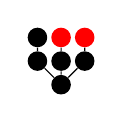
\begin{tikzpicture}[scale=.2]
\node[circle, scale=0.75, fill] (tid0) at (2.25,0){};
\node[circle, scale=0.75, fill] (tid1) at (0.75,1.5){};
\node[circle, scale=0.75, fill] (tid4) at (0.75,3){};

\draw[](tid1) -- (tid4);

\node[circle, scale=0.75, fill] (tid2) at (2.25,1.5){};
\node[circle, scale=0.75, fill, red] (tid5) at (2.25,3){};

\draw[](tid2) -- (tid5);

\node[circle, scale=0.75, fill] (tid3) at (3.75,1.5){};
\node[circle, scale=0.75, fill, red] (tid6) at (3.75,3){};

\draw[](tid3) -- (tid6);

\draw[](tid0) -- (tid1);
\draw[](tid0) -- (tid2);
\draw[](tid0) -- (tid3);

\end{tikzpicture}
};
\draw (sn0x9a6d1a0W18.south) -- (sn0x9a6d750W9.north);
\node[draw=black] (sn0x9a6d4b8W27) at (27, -40) {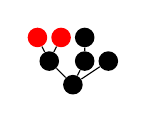
\begin{tikzpicture}[scale=.2]
\node[circle, scale=0.75, fill] (tid0) at (3,0){};
\node[circle, scale=0.75, fill] (tid1) at (1.5,1.5){};
\node[circle, scale=0.75, fill, red] (tid4) at (0.75,3){};

\node[circle, scale=0.75, fill, red] (tid5) at (2.25,3){};

\draw[](tid1) -- (tid4);
\draw[](tid1) -- (tid5);

\node[circle, scale=0.75, fill] (tid2) at (3.75,1.5){};
\node[circle, scale=0.75, fill] (tid6) at (3.75,3){};

\draw[](tid2) -- (tid6);

\node[circle, scale=0.75, fill] (tid3) at (5.25,1.5){};

\draw[](tid0) -- (tid1);
\draw[](tid0) -- (tid2);
\draw[](tid0) -- (tid3);

\end{tikzpicture}
};
\draw (sn0x9a6d4b8W27.south) -- (sn0x9a6d750W9.north);
\node[draw=black] (sn0x9a6d520W36) at (36, -40) {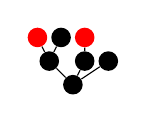
\begin{tikzpicture}[scale=.2]
\node[circle, scale=0.75, fill] (tid0) at (3,0){};
\node[circle, scale=0.75, fill] (tid1) at (1.5,1.5){};
\node[circle, scale=0.75, fill, red] (tid4) at (0.75,3){};

\node[circle, scale=0.75, fill] (tid5) at (2.25,3){};

\draw[](tid1) -- (tid4);
\draw[](tid1) -- (tid5);

\node[circle, scale=0.75, fill] (tid2) at (3.75,1.5){};
\node[circle, scale=0.75, fill, red] (tid6) at (3.75,3){};

\draw[](tid2) -- (tid6);

\node[circle, scale=0.75, fill] (tid3) at (5.25,1.5){};

\draw[](tid0) -- (tid1);
\draw[](tid0) -- (tid2);
\draw[](tid0) -- (tid3);

\end{tikzpicture}
};
\node[draw=black] (sn0x9a6e378W18) at (18, -50) {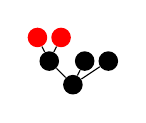
\begin{tikzpicture}[scale=.2]
\node[circle, scale=0.75, fill] (tid0) at (3,0){};
\node[circle, scale=0.75, fill] (tid1) at (1.5,1.5){};
\node[circle, scale=0.75, fill, red] (tid4) at (0.75,3){};

\node[circle, scale=0.75, fill, red] (tid5) at (2.25,3){};

\draw[](tid1) -- (tid4);
\draw[](tid1) -- (tid5);

\node[circle, scale=0.75, fill] (tid2) at (3.75,1.5){};

\node[circle, scale=0.75, fill] (tid3) at (5.25,1.5){};

\draw[](tid0) -- (tid1);
\draw[](tid0) -- (tid2);
\draw[](tid0) -- (tid3);

\end{tikzpicture}
};
\draw (sn0x9a6e378W18.south) -- (sn0x9a6da10W9.north);
\draw (sn0x9a6d520W36.south) -- (sn0x9a6d750W9.north);
\draw (sn0x9a6d520W36.south) -- (sn0x9a6e378W18.north);
\draw (sn0x9a696c8W9.south) -- (sn0x9a6cfd8W9.north);
\draw (sn0x9a696c8W9.south) -- (sn0x9a6d1a0W18.north);
\draw (sn0x9a696c8W9.south) -- (sn0x9a6d4b8W27.north);
\draw (sn0x9a696c8W9.south) -- (sn0x9a6d520W36.north);
\node[draw=black] (sn0x9a68588W18) at (18, -30) {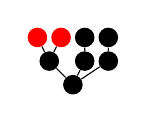
\begin{tikzpicture}[scale=.2]
\node[circle, scale=0.75, fill] (tid0) at (3,0){};
\node[circle, scale=0.75, fill] (tid1) at (1.5,1.5){};
\node[circle, scale=0.75, fill, red] (tid4) at (0.75,3){};

\node[circle, scale=0.75, fill, red] (tid5) at (2.25,3){};

\draw[](tid1) -- (tid4);
\draw[](tid1) -- (tid5);

\node[circle, scale=0.75, fill] (tid2) at (3.75,1.5){};
\node[circle, scale=0.75, fill] (tid6) at (3.75,3){};

\draw[](tid2) -- (tid6);

\node[circle, scale=0.75, fill] (tid3) at (5.25,1.5){};
\node[circle, scale=0.75, fill] (tid7) at (5.25,3){};

\draw[](tid3) -- (tid7);

\draw[](tid0) -- (tid1);
\draw[](tid0) -- (tid2);
\draw[](tid0) -- (tid3);

\end{tikzpicture}
};
\node[draw=black] (sn0x9a6ed08W45) at (45, -40) {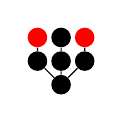
\begin{tikzpicture}[scale=.2]
\node[circle, scale=0.75, fill] (tid0) at (2.25,0){};
\node[circle, scale=0.75, fill] (tid1) at (0.75,1.5){};
\node[circle, scale=0.75, fill, red] (tid4) at (0.75,3){};

\draw[](tid1) -- (tid4);

\node[circle, scale=0.75, fill] (tid2) at (2.25,1.5){};
\node[circle, scale=0.75, fill] (tid5) at (2.25,3){};

\draw[](tid2) -- (tid5);

\node[circle, scale=0.75, fill] (tid3) at (3.75,1.5){};
\node[circle, scale=0.75, fill, red] (tid6) at (3.75,3){};

\draw[](tid3) -- (tid6);

\draw[](tid0) -- (tid1);
\draw[](tid0) -- (tid2);
\draw[](tid0) -- (tid3);

\end{tikzpicture}
};
\draw (sn0x9a6ed08W45.south) -- (sn0x9a6d750W9.north);
\draw (sn0x9a68588W18.south) -- (sn0x9a6cfd8W9.north);
\draw (sn0x9a68588W18.south) -- (sn0x9a6ed08W45.north);
\node[draw=black] (sn0x9a69108W27) at (27, -30) {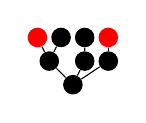
\begin{tikzpicture}[scale=.2]
\node[circle, scale=0.75, fill] (tid0) at (3,0){};
\node[circle, scale=0.75, fill] (tid1) at (1.5,1.5){};
\node[circle, scale=0.75, fill, red] (tid4) at (0.75,3){};

\node[circle, scale=0.75, fill] (tid5) at (2.25,3){};

\draw[](tid1) -- (tid4);
\draw[](tid1) -- (tid5);

\node[circle, scale=0.75, fill] (tid2) at (3.75,1.5){};
\node[circle, scale=0.75, fill] (tid6) at (3.75,3){};

\draw[](tid2) -- (tid6);

\node[circle, scale=0.75, fill] (tid3) at (5.25,1.5){};
\node[circle, scale=0.75, fill, red] (tid7) at (5.25,3){};

\draw[](tid3) -- (tid7);

\draw[](tid0) -- (tid1);
\draw[](tid0) -- (tid2);
\draw[](tid0) -- (tid3);

\end{tikzpicture}
};
\draw (sn0x9a69108W27.south) -- (sn0x9a6ed08W45.north);
\draw (sn0x9a69108W27.south) -- (sn0x9a6d1a0W18.north);
\draw (sn0x9a69108W27.south) -- (sn0x9a6d4b8W27.north);
\draw (sn0x9a69108W27.south) -- (sn0x9a6d520W36.north);
\draw (sn0x9a68730W9.south) -- (sn0x9a696c8W9.north);
\draw (sn0x9a68730W9.south) -- (sn0x9a68588W18.north);
\draw (sn0x9a68730W9.south) -- (sn0x9a69108W27.north);
\node[draw=black] (sn0x9a67428W18) at (18, -20) {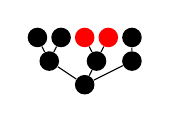
\begin{tikzpicture}[scale=.2]
\node[circle, scale=0.75, fill] (tid0) at (3.75,0){};
\node[circle, scale=0.75, fill] (tid1) at (1.5,1.5){};
\node[circle, scale=0.75, fill] (tid4) at (0.75,3){};

\node[circle, scale=0.75, fill] (tid5) at (2.25,3){};

\draw[](tid1) -- (tid4);
\draw[](tid1) -- (tid5);

\node[circle, scale=0.75, fill] (tid2) at (4.5,1.5){};
\node[circle, scale=0.75, fill, red] (tid6) at (3.75,3){};

\node[circle, scale=0.75, fill, red] (tid7) at (5.25,3){};

\draw[](tid2) -- (tid6);
\draw[](tid2) -- (tid7);

\node[circle, scale=0.75, fill] (tid3) at (6.75,1.5){};
\node[circle, scale=0.75, fill] (tid8) at (6.75,3){};

\draw[](tid3) -- (tid8);

\draw[](tid0) -- (tid1);
\draw[](tid0) -- (tid2);
\draw[](tid0) -- (tid3);

\end{tikzpicture}
};
\node[draw=black] (sn0x9a6ef58W36) at (36, -30) {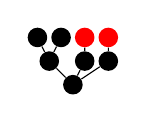
\begin{tikzpicture}[scale=.2]
\node[circle, scale=0.75, fill] (tid0) at (3,0){};
\node[circle, scale=0.75, fill] (tid1) at (1.5,1.5){};
\node[circle, scale=0.75, fill] (tid4) at (0.75,3){};

\node[circle, scale=0.75, fill] (tid5) at (2.25,3){};

\draw[](tid1) -- (tid4);
\draw[](tid1) -- (tid5);

\node[circle, scale=0.75, fill] (tid2) at (3.75,1.5){};
\node[circle, scale=0.75, fill, red] (tid6) at (3.75,3){};

\draw[](tid2) -- (tid6);

\node[circle, scale=0.75, fill] (tid3) at (5.25,1.5){};
\node[circle, scale=0.75, fill, red] (tid7) at (5.25,3){};

\draw[](tid3) -- (tid7);

\draw[](tid0) -- (tid1);
\draw[](tid0) -- (tid2);
\draw[](tid0) -- (tid3);

\end{tikzpicture}
};
\draw (sn0x9a6ef58W36.south) -- (sn0x9a6d520W36.north);
\draw (sn0x9a67428W18.south) -- (sn0x9a696c8W9.north);
\draw (sn0x9a67428W18.south) -- (sn0x9a6ef58W36.north);
\node[draw=black] (sn0x9a69cd8W27) at (27, -20) {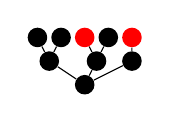
\begin{tikzpicture}[scale=.2]
\node[circle, scale=0.75, fill] (tid0) at (3.75,0){};
\node[circle, scale=0.75, fill] (tid1) at (1.5,1.5){};
\node[circle, scale=0.75, fill] (tid4) at (0.75,3){};

\node[circle, scale=0.75, fill] (tid5) at (2.25,3){};

\draw[](tid1) -- (tid4);
\draw[](tid1) -- (tid5);

\node[circle, scale=0.75, fill] (tid2) at (4.5,1.5){};
\node[circle, scale=0.75, fill, red] (tid6) at (3.75,3){};

\node[circle, scale=0.75, fill] (tid7) at (5.25,3){};

\draw[](tid2) -- (tid6);
\draw[](tid2) -- (tid7);

\node[circle, scale=0.75, fill] (tid3) at (6.75,1.5){};
\node[circle, scale=0.75, fill, red] (tid8) at (6.75,3){};

\draw[](tid3) -- (tid8);

\draw[](tid0) -- (tid1);
\draw[](tid0) -- (tid2);
\draw[](tid0) -- (tid3);

\end{tikzpicture}
};
\node[draw=black] (sn0x9a6f1b0W45) at (45, -30) {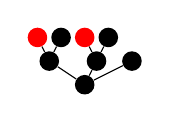
\begin{tikzpicture}[scale=.2]
\node[circle, scale=0.75, fill] (tid0) at (3.75,0){};
\node[circle, scale=0.75, fill] (tid1) at (1.5,1.5){};
\node[circle, scale=0.75, fill, red] (tid4) at (0.75,3){};

\node[circle, scale=0.75, fill] (tid5) at (2.25,3){};

\draw[](tid1) -- (tid4);
\draw[](tid1) -- (tid5);

\node[circle, scale=0.75, fill] (tid2) at (4.5,1.5){};
\node[circle, scale=0.75, fill, red] (tid6) at (3.75,3){};

\node[circle, scale=0.75, fill] (tid7) at (5.25,3){};

\draw[](tid2) -- (tid6);
\draw[](tid2) -- (tid7);

\node[circle, scale=0.75, fill] (tid3) at (6.75,1.5){};

\draw[](tid0) -- (tid1);
\draw[](tid0) -- (tid2);
\draw[](tid0) -- (tid3);

\end{tikzpicture}
};
\draw (sn0x9a6f1b0W45.south) -- (sn0x9a6d520W36.north);
\draw (sn0x9a6f1b0W45.south) -- (sn0x9a6d4b8W27.north);
\node[draw=black] (sn0x9a6f4c0W54) at (54, -30) {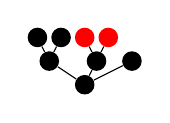
\begin{tikzpicture}[scale=.2]
\node[circle, scale=0.75, fill] (tid0) at (3.75,0){};
\node[circle, scale=0.75, fill] (tid1) at (1.5,1.5){};
\node[circle, scale=0.75, fill] (tid4) at (0.75,3){};

\node[circle, scale=0.75, fill] (tid5) at (2.25,3){};

\draw[](tid1) -- (tid4);
\draw[](tid1) -- (tid5);

\node[circle, scale=0.75, fill] (tid2) at (4.5,1.5){};
\node[circle, scale=0.75, fill, red] (tid6) at (3.75,3){};

\node[circle, scale=0.75, fill, red] (tid7) at (5.25,3){};

\draw[](tid2) -- (tid6);
\draw[](tid2) -- (tid7);

\node[circle, scale=0.75, fill] (tid3) at (6.75,1.5){};

\draw[](tid0) -- (tid1);
\draw[](tid0) -- (tid2);
\draw[](tid0) -- (tid3);

\end{tikzpicture}
};
\draw (sn0x9a6f4c0W54.south) -- (sn0x9a6d520W36.north);
\draw (sn0x9a69cd8W27.south) -- (sn0x9a69108W27.north);
\draw (sn0x9a69cd8W27.south) -- (sn0x9a6ef58W36.north);
\draw (sn0x9a69cd8W27.south) -- (sn0x9a6f1b0W45.north);
\draw (sn0x9a69cd8W27.south) -- (sn0x9a6f4c0W54.north);
\node[draw=black] (sn0x9a67c98W36) at (36, -20) {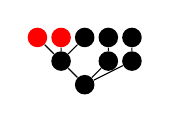
\begin{tikzpicture}[scale=.2]
\node[circle, scale=0.75, fill] (tid0) at (3.75,0){};
\node[circle, scale=0.75, fill] (tid1) at (2.25,1.5){};
\node[circle, scale=0.75, fill, red] (tid4) at (0.75,3){};

\node[circle, scale=0.75, fill, red] (tid5) at (2.25,3){};

\node[circle, scale=0.75, fill] (tid6) at (3.75,3){};

\draw[](tid1) -- (tid4);
\draw[](tid1) -- (tid5);
\draw[](tid1) -- (tid6);

\node[circle, scale=0.75, fill] (tid2) at (5.25,1.5){};
\node[circle, scale=0.75, fill] (tid7) at (5.25,3){};

\draw[](tid2) -- (tid7);

\node[circle, scale=0.75, fill] (tid3) at (6.75,1.5){};
\node[circle, scale=0.75, fill] (tid8) at (6.75,3){};

\draw[](tid3) -- (tid8);

\draw[](tid0) -- (tid1);
\draw[](tid0) -- (tid2);
\draw[](tid0) -- (tid3);

\end{tikzpicture}
};
\draw (sn0x9a67c98W36.south) -- (sn0x9a68588W18.north);
\draw (sn0x9a67c98W36.south) -- (sn0x9a696c8W9.north);
\draw (sn0x9a67c98W36.south) -- (sn0x9a69108W27.north);
\node[draw=black] (sn0x9a697e0W45) at (45, -20) {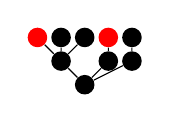
\begin{tikzpicture}[scale=.2]
\node[circle, scale=0.75, fill] (tid0) at (3.75,0){};
\node[circle, scale=0.75, fill] (tid1) at (2.25,1.5){};
\node[circle, scale=0.75, fill, red] (tid4) at (0.75,3){};

\node[circle, scale=0.75, fill] (tid5) at (2.25,3){};

\node[circle, scale=0.75, fill] (tid6) at (3.75,3){};

\draw[](tid1) -- (tid4);
\draw[](tid1) -- (tid5);
\draw[](tid1) -- (tid6);

\node[circle, scale=0.75, fill] (tid2) at (5.25,1.5){};
\node[circle, scale=0.75, fill, red] (tid7) at (5.25,3){};

\draw[](tid2) -- (tid7);

\node[circle, scale=0.75, fill] (tid3) at (6.75,1.5){};
\node[circle, scale=0.75, fill] (tid8) at (6.75,3){};

\draw[](tid3) -- (tid8);

\draw[](tid0) -- (tid1);
\draw[](tid0) -- (tid2);
\draw[](tid0) -- (tid3);

\end{tikzpicture}
};
\node[draw=black] (sn0x9a6f8b0W63) at (63, -30) {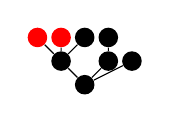
\begin{tikzpicture}[scale=.2]
\node[circle, scale=0.75, fill] (tid0) at (3.75,0){};
\node[circle, scale=0.75, fill] (tid1) at (2.25,1.5){};
\node[circle, scale=0.75, fill, red] (tid4) at (0.75,3){};

\node[circle, scale=0.75, fill, red] (tid5) at (2.25,3){};

\node[circle, scale=0.75, fill] (tid6) at (3.75,3){};

\draw[](tid1) -- (tid4);
\draw[](tid1) -- (tid5);
\draw[](tid1) -- (tid6);

\node[circle, scale=0.75, fill] (tid2) at (5.25,1.5){};
\node[circle, scale=0.75, fill] (tid7) at (5.25,3){};

\draw[](tid2) -- (tid7);

\node[circle, scale=0.75, fill] (tid3) at (6.75,1.5){};

\draw[](tid0) -- (tid1);
\draw[](tid0) -- (tid2);
\draw[](tid0) -- (tid3);

\end{tikzpicture}
};
\draw (sn0x9a6f8b0W63.south) -- (sn0x9a6d4b8W27.north);
\draw (sn0x9a6f8b0W63.south) -- (sn0x9a6d520W36.north);
\node[draw=black] (sn0x9a6fc50W72) at (72, -30) {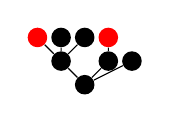
\begin{tikzpicture}[scale=.2]
\node[circle, scale=0.75, fill] (tid0) at (3.75,0){};
\node[circle, scale=0.75, fill] (tid1) at (2.25,1.5){};
\node[circle, scale=0.75, fill, red] (tid4) at (0.75,3){};

\node[circle, scale=0.75, fill] (tid5) at (2.25,3){};

\node[circle, scale=0.75, fill] (tid6) at (3.75,3){};

\draw[](tid1) -- (tid4);
\draw[](tid1) -- (tid5);
\draw[](tid1) -- (tid6);

\node[circle, scale=0.75, fill] (tid2) at (5.25,1.5){};
\node[circle, scale=0.75, fill, red] (tid7) at (5.25,3){};

\draw[](tid2) -- (tid7);

\node[circle, scale=0.75, fill] (tid3) at (6.75,1.5){};

\draw[](tid0) -- (tid1);
\draw[](tid0) -- (tid2);
\draw[](tid0) -- (tid3);

\end{tikzpicture}
};
\node[draw=black] (sn0x9a6fe48W54) at (54, -40) {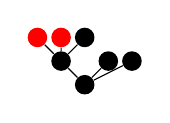
\begin{tikzpicture}[scale=.2]
\node[circle, scale=0.75, fill] (tid0) at (3.75,0){};
\node[circle, scale=0.75, fill] (tid1) at (2.25,1.5){};
\node[circle, scale=0.75, fill, red] (tid4) at (0.75,3){};

\node[circle, scale=0.75, fill, red] (tid5) at (2.25,3){};

\node[circle, scale=0.75, fill] (tid6) at (3.75,3){};

\draw[](tid1) -- (tid4);
\draw[](tid1) -- (tid5);
\draw[](tid1) -- (tid6);

\node[circle, scale=0.75, fill] (tid2) at (5.25,1.5){};

\node[circle, scale=0.75, fill] (tid3) at (6.75,1.5){};

\draw[](tid0) -- (tid1);
\draw[](tid0) -- (tid2);
\draw[](tid0) -- (tid3);

\end{tikzpicture}
};
\draw (sn0x9a6fe48W54.south) -- (sn0x9a6e378W18.north);
\draw (sn0x9a6fc50W72.south) -- (sn0x9a6d520W36.north);
\draw (sn0x9a6fc50W72.south) -- (sn0x9a6fe48W54.north);
\draw (sn0x9a697e0W45.south) -- (sn0x9a696c8W9.north);
\draw (sn0x9a697e0W45.south) -- (sn0x9a6ef58W36.north);
\draw (sn0x9a697e0W45.south) -- (sn0x9a6f8b0W63.north);
\draw (sn0x9a697e0W45.south) -- (sn0x9a6fc50W72.north);
\node[draw=black] (sn0x9a69aa8W54) at (54, -20) {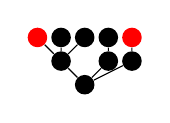
\begin{tikzpicture}[scale=.2]
\node[circle, scale=0.75, fill] (tid0) at (3.75,0){};
\node[circle, scale=0.75, fill] (tid1) at (2.25,1.5){};
\node[circle, scale=0.75, fill, red] (tid4) at (0.75,3){};

\node[circle, scale=0.75, fill] (tid5) at (2.25,3){};

\node[circle, scale=0.75, fill] (tid6) at (3.75,3){};

\draw[](tid1) -- (tid4);
\draw[](tid1) -- (tid5);
\draw[](tid1) -- (tid6);

\node[circle, scale=0.75, fill] (tid2) at (5.25,1.5){};
\node[circle, scale=0.75, fill] (tid7) at (5.25,3){};

\draw[](tid2) -- (tid7);

\node[circle, scale=0.75, fill] (tid3) at (6.75,1.5){};
\node[circle, scale=0.75, fill, red] (tid8) at (6.75,3){};

\draw[](tid3) -- (tid8);

\draw[](tid0) -- (tid1);
\draw[](tid0) -- (tid2);
\draw[](tid0) -- (tid3);

\end{tikzpicture}
};
\draw (sn0x9a69aa8W54.south) -- (sn0x9a69108W27.north);
\draw (sn0x9a69aa8W54.south) -- (sn0x9a6ef58W36.north);
\draw (sn0x9a69aa8W54.south) -- (sn0x9a6f8b0W63.north);
\draw (sn0x9a69aa8W54.south) -- (sn0x9a6fc50W72.north);
\draw (sn0x9a68990W9.south) -- (sn0x9a68730W9.north);
\draw (sn0x9a68990W9.south) -- (sn0x9a67428W18.north);
\draw (sn0x9a68990W9.south) -- (sn0x9a69cd8W27.north);
\draw (sn0x9a68990W9.south) -- (sn0x9a67c98W36.north);
\draw (sn0x9a68990W9.south) -- (sn0x9a697e0W45.north);
\draw (sn0x9a68990W9.south) -- (sn0x9a69aa8W54.north);
\end{tikzpicture}

%%% Local Variables:
%%% TeX-master: "thesis/thesis.tex"
%%% End: 

\begin{tikzpicture}[scale=.2, anchor=base]
\node[draw=black] (sn0x9a689f0W9) at (9, -10) {\begin{tikzpicture}[scale=.2]
\node[circle, scale=0.75, fill] (tid0) at (4.5,0){};
\node[circle, scale=0.75, fill] (tid1) at (2.25,1.5){};
\node[circle, scale=0.75, fill, red] (tid4) at (0.75,3){};

\node[circle, scale=0.75, fill, red] (tid5) at (2.25,3){};

\node[circle, scale=0.75, fill] (tid6) at (3.75,3){};

\draw[](tid1) -- (tid4);
\draw[](tid1) -- (tid5);
\draw[](tid1) -- (tid6);

\node[circle, scale=0.75, fill] (tid2) at (6,1.5){};
\node[circle, scale=0.75, fill] (tid7) at (5.25,3){};

\node[circle, scale=0.75, fill] (tid8) at (6.75,3){};

\draw[](tid2) -- (tid7);
\draw[](tid2) -- (tid8);

\node[circle, scale=0.75, fill] (tid3) at (8.25,1.5){};
\node[circle, scale=0.75, fill] (tid9) at (8.25,3){};

\draw[](tid3) -- (tid9);

\draw[](tid0) -- (tid1);
\draw[](tid0) -- (tid2);
\draw[](tid0) -- (tid3);

\end{tikzpicture}
};
\node[draw=black] (sn0x9a70650W9) at (9, -20) {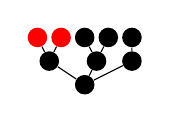
\begin{tikzpicture}[scale=.2]
\node[circle, scale=0.75, fill] (tid0) at (3.75,0){};
\node[circle, scale=0.75, fill] (tid1) at (1.5,1.5){};
\node[circle, scale=0.75, fill, red] (tid4) at (0.75,3){};

\node[circle, scale=0.75, fill, red] (tid5) at (2.25,3){};

\draw[](tid1) -- (tid4);
\draw[](tid1) -- (tid5);

\node[circle, scale=0.75, fill] (tid2) at (4.5,1.5){};
\node[circle, scale=0.75, fill] (tid6) at (3.75,3){};

\node[circle, scale=0.75, fill] (tid7) at (5.25,3){};

\draw[](tid2) -- (tid6);
\draw[](tid2) -- (tid7);

\node[circle, scale=0.75, fill] (tid3) at (6.75,1.5){};
\node[circle, scale=0.75, fill] (tid8) at (6.75,3){};

\draw[](tid3) -- (tid8);

\draw[](tid0) -- (tid1);
\draw[](tid0) -- (tid2);
\draw[](tid0) -- (tid3);

\end{tikzpicture}
};
\node[draw=black] (sn0x9a696c8W9) at (9, -30) {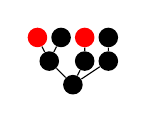
\begin{tikzpicture}[scale=.2]
\node[circle, scale=0.75, fill] (tid0) at (3,0){};
\node[circle, scale=0.75, fill] (tid1) at (1.5,1.5){};
\node[circle, scale=0.75, fill, red] (tid4) at (0.75,3){};

\node[circle, scale=0.75, fill] (tid5) at (2.25,3){};

\draw[](tid1) -- (tid4);
\draw[](tid1) -- (tid5);

\node[circle, scale=0.75, fill] (tid2) at (3.75,1.5){};
\node[circle, scale=0.75, fill, red] (tid6) at (3.75,3){};

\draw[](tid2) -- (tid6);

\node[circle, scale=0.75, fill] (tid3) at (5.25,1.5){};
\node[circle, scale=0.75, fill] (tid7) at (5.25,3){};

\draw[](tid3) -- (tid7);

\draw[](tid0) -- (tid1);
\draw[](tid0) -- (tid2);
\draw[](tid0) -- (tid3);

\end{tikzpicture}
};
\node[draw=black] (sn0x9a6cfd8W9) at (9, -40) {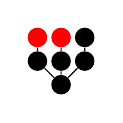
\begin{tikzpicture}[scale=.2]
\node[circle, scale=0.75, fill] (tid0) at (2.25,0){};
\node[circle, scale=0.75, fill] (tid1) at (0.75,1.5){};
\node[circle, scale=0.75, fill, red] (tid4) at (0.75,3){};

\draw[](tid1) -- (tid4);

\node[circle, scale=0.75, fill] (tid2) at (2.25,1.5){};
\node[circle, scale=0.75, fill, red] (tid5) at (2.25,3){};

\draw[](tid2) -- (tid5);

\node[circle, scale=0.75, fill] (tid3) at (3.75,1.5){};
\node[circle, scale=0.75, fill] (tid6) at (3.75,3){};

\draw[](tid3) -- (tid6);

\draw[](tid0) -- (tid1);
\draw[](tid0) -- (tid2);
\draw[](tid0) -- (tid3);

\end{tikzpicture}
};
\node[draw=black] (sn0x9a6d750W9) at (9, -50) {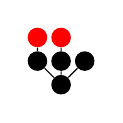
\begin{tikzpicture}[scale=.2]
\node[circle, scale=0.75, fill] (tid0) at (2.25,0){};
\node[circle, scale=0.75, fill] (tid1) at (0.75,1.5){};
\node[circle, scale=0.75, fill, red] (tid4) at (0.75,3){};

\draw[](tid1) -- (tid4);

\node[circle, scale=0.75, fill] (tid2) at (2.25,1.5){};
\node[circle, scale=0.75, fill, red] (tid5) at (2.25,3){};

\draw[](tid2) -- (tid5);

\node[circle, scale=0.75, fill] (tid3) at (3.75,1.5){};

\draw[](tid0) -- (tid1);
\draw[](tid0) -- (tid2);
\draw[](tid0) -- (tid3);

\end{tikzpicture}
};
\node[draw=black] (sn0x9a6da10W9) at (9, -60) {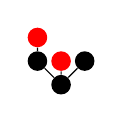
\begin{tikzpicture}[scale=.2]
\node[circle, scale=0.75, fill] (tid0) at (2.25,0){};
\node[circle, scale=0.75, fill] (tid1) at (0.75,1.5){};
\node[circle, scale=0.75, fill, red] (tid4) at (0.75,3){};

\draw[](tid1) -- (tid4);

\node[circle, scale=0.75, fill, red] (tid2) at (2.25,1.5){};

\node[circle, scale=0.75, fill] (tid3) at (3.75,1.5){};

\draw[](tid0) -- (tid1);
\draw[](tid0) -- (tid2);
\draw[](tid0) -- (tid3);

\end{tikzpicture}
};
\node[draw=black] (sn0x9a6d990W9) at (9, -70) {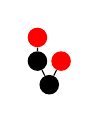
\begin{tikzpicture}[scale=.2]
\node[circle, scale=0.75, fill] (tid0) at (1.5,0){};
\node[circle, scale=0.75, fill] (tid1) at (0.75,1.5){};
\node[circle, scale=0.75, fill, red] (tid3) at (0.75,3){};

\draw[](tid1) -- (tid3);

\node[circle, scale=0.75, fill, red] (tid2) at (2.25,1.5){};

\draw[](tid0) -- (tid1);
\draw[](tid0) -- (tid2);

\end{tikzpicture}
};
\node[draw=black] (sn0x9a6dd40W9) at (9, -80) {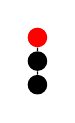
\begin{tikzpicture}[scale=.2]
\node[circle, scale=0.75, fill] (tid0) at (0.75,0){};
\node[circle, scale=0.75, fill] (tid1) at (0.75,1.5){};
\node[circle, scale=0.75, fill, red] (tid2) at (0.75,3){};

\draw[](tid1) -- (tid2);

\draw[](tid0) -- (tid1);

\end{tikzpicture}
};
\node[draw=black] (sn0x9a6e148W9) at (9, -90) {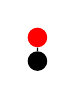
\begin{tikzpicture}[scale=.2]
\node[circle, scale=0.75, fill] (tid0) at (0.75,0){};
\node[circle, scale=0.75, fill, red] (tid1) at (0.75,1.5){};

\draw[](tid0) -- (tid1);

\end{tikzpicture}
};
\node[draw=black] (sn0x9a6e1b0W9) at (9, -100) {
\begin{tikzpicture}[scale=.2]
\node[circle, scale=0.75, fill] (tid0) at (0.75,0){};

\end{tikzpicture}
};
\draw (sn0x9a6e148W9.south) -- (sn0x9a6e1b0W9.north);
\draw (sn0x9a6dd40W9.south) -- (sn0x9a6e148W9.north);
\node[draw=black] (sn0x9a6dff8W18) at (18, -80) {
\begin{tikzpicture}[scale=.2]
\node[circle, scale=0.75, fill] (tid0) at (1.5,0){};
\node[circle, scale=0.75, fill, red] (tid1) at (0.75,1.5){};

\node[circle, scale=0.75, fill, red] (tid2) at (2.25,1.5){};

\draw[](tid0) -- (tid1);
\draw[](tid0) -- (tid2);

\end{tikzpicture}
};
\draw (sn0x9a6dff8W18.south) -- (sn0x9a6e148W9.north);
\draw (sn0x9a6d990W9.south) -- (sn0x9a6dd40W9.north);
\draw (sn0x9a6d990W9.south) -- (sn0x9a6dff8W18.north);
\node[draw=black] (sn0x9a6dcd8W18) at (18, -70) {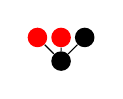
\begin{tikzpicture}[scale=.2]
\node[circle, scale=0.75, fill] (tid0) at (2.25,0){};
\node[circle, scale=0.75, fill, red] (tid1) at (0.75,1.5){};

\node[circle, scale=0.75, fill, red] (tid2) at (2.25,1.5){};

\node[circle, scale=0.75, fill] (tid3) at (3.75,1.5){};

\draw[](tid0) -- (tid1);
\draw[](tid0) -- (tid2);
\draw[](tid0) -- (tid3);

\end{tikzpicture}
};
\draw (sn0x9a6dcd8W18.south) -- (sn0x9a6dff8W18.north);
\draw (sn0x9a6da10W9.south) -- (sn0x9a6d990W9.north);
\draw (sn0x9a6da10W9.south) -- (sn0x9a6dcd8W18.north);
\draw (sn0x9a6d750W9.south) -- (sn0x9a6da10W9.north);
\draw (sn0x9a6cfd8W9.south) -- (sn0x9a6d750W9.north);
\node[draw=black] (sn0x9a6d1a0W18) at (18, -40) {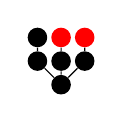
\begin{tikzpicture}[scale=.2]
\node[circle, scale=0.75, fill] (tid0) at (2.25,0){};
\node[circle, scale=0.75, fill] (tid1) at (0.75,1.5){};
\node[circle, scale=0.75, fill] (tid4) at (0.75,3){};

\draw[](tid1) -- (tid4);

\node[circle, scale=0.75, fill] (tid2) at (2.25,1.5){};
\node[circle, scale=0.75, fill, red] (tid5) at (2.25,3){};

\draw[](tid2) -- (tid5);

\node[circle, scale=0.75, fill] (tid3) at (3.75,1.5){};
\node[circle, scale=0.75, fill, red] (tid6) at (3.75,3){};

\draw[](tid3) -- (tid6);

\draw[](tid0) -- (tid1);
\draw[](tid0) -- (tid2);
\draw[](tid0) -- (tid3);

\end{tikzpicture}
};
\draw (sn0x9a6d1a0W18.south) -- (sn0x9a6d750W9.north);
\node[draw=black] (sn0x9a6d4b8W27) at (27, -40) {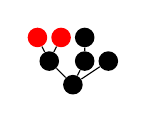
\begin{tikzpicture}[scale=.2]
\node[circle, scale=0.75, fill] (tid0) at (3,0){};
\node[circle, scale=0.75, fill] (tid1) at (1.5,1.5){};
\node[circle, scale=0.75, fill, red] (tid4) at (0.75,3){};

\node[circle, scale=0.75, fill, red] (tid5) at (2.25,3){};

\draw[](tid1) -- (tid4);
\draw[](tid1) -- (tid5);

\node[circle, scale=0.75, fill] (tid2) at (3.75,1.5){};
\node[circle, scale=0.75, fill] (tid6) at (3.75,3){};

\draw[](tid2) -- (tid6);

\node[circle, scale=0.75, fill] (tid3) at (5.25,1.5){};

\draw[](tid0) -- (tid1);
\draw[](tid0) -- (tid2);
\draw[](tid0) -- (tid3);

\end{tikzpicture}
};
\draw (sn0x9a6d4b8W27.south) -- (sn0x9a6d750W9.north);
\node[draw=black] (sn0x9a6d520W36) at (36, -40) {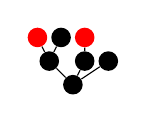
\begin{tikzpicture}[scale=.2]
\node[circle, scale=0.75, fill] (tid0) at (3,0){};
\node[circle, scale=0.75, fill] (tid1) at (1.5,1.5){};
\node[circle, scale=0.75, fill, red] (tid4) at (0.75,3){};

\node[circle, scale=0.75, fill] (tid5) at (2.25,3){};

\draw[](tid1) -- (tid4);
\draw[](tid1) -- (tid5);

\node[circle, scale=0.75, fill] (tid2) at (3.75,1.5){};
\node[circle, scale=0.75, fill, red] (tid6) at (3.75,3){};

\draw[](tid2) -- (tid6);

\node[circle, scale=0.75, fill] (tid3) at (5.25,1.5){};

\draw[](tid0) -- (tid1);
\draw[](tid0) -- (tid2);
\draw[](tid0) -- (tid3);

\end{tikzpicture}
};
\node[draw=black] (sn0x9a6e378W18) at (18, -50) {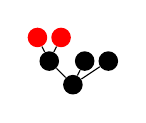
\begin{tikzpicture}[scale=.2]
\node[circle, scale=0.75, fill] (tid0) at (3,0){};
\node[circle, scale=0.75, fill] (tid1) at (1.5,1.5){};
\node[circle, scale=0.75, fill, red] (tid4) at (0.75,3){};

\node[circle, scale=0.75, fill, red] (tid5) at (2.25,3){};

\draw[](tid1) -- (tid4);
\draw[](tid1) -- (tid5);

\node[circle, scale=0.75, fill] (tid2) at (3.75,1.5){};

\node[circle, scale=0.75, fill] (tid3) at (5.25,1.5){};

\draw[](tid0) -- (tid1);
\draw[](tid0) -- (tid2);
\draw[](tid0) -- (tid3);

\end{tikzpicture}
};
\draw (sn0x9a6e378W18.south) -- (sn0x9a6da10W9.north);
\draw (sn0x9a6d520W36.south) -- (sn0x9a6d750W9.north);
\draw (sn0x9a6d520W36.south) -- (sn0x9a6e378W18.north);
\draw (sn0x9a696c8W9.south) -- (sn0x9a6cfd8W9.north);
\draw (sn0x9a696c8W9.south) -- (sn0x9a6d1a0W18.north);
\draw (sn0x9a696c8W9.south) -- (sn0x9a6d4b8W27.north);
\draw (sn0x9a696c8W9.south) -- (sn0x9a6d520W36.north);
\node[draw=black] (sn0x9a6ef58W18) at (18, -30) {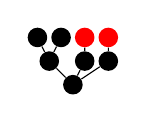
\begin{tikzpicture}[scale=.2]
\node[circle, scale=0.75, fill] (tid0) at (3,0){};
\node[circle, scale=0.75, fill] (tid1) at (1.5,1.5){};
\node[circle, scale=0.75, fill] (tid4) at (0.75,3){};

\node[circle, scale=0.75, fill] (tid5) at (2.25,3){};

\draw[](tid1) -- (tid4);
\draw[](tid1) -- (tid5);

\node[circle, scale=0.75, fill] (tid2) at (3.75,1.5){};
\node[circle, scale=0.75, fill, red] (tid6) at (3.75,3){};

\draw[](tid2) -- (tid6);

\node[circle, scale=0.75, fill] (tid3) at (5.25,1.5){};
\node[circle, scale=0.75, fill, red] (tid7) at (5.25,3){};

\draw[](tid3) -- (tid7);

\draw[](tid0) -- (tid1);
\draw[](tid0) -- (tid2);
\draw[](tid0) -- (tid3);

\end{tikzpicture}
};
\draw (sn0x9a6ef58W18.south) -- (sn0x9a6d520W36.north);
\draw (sn0x9a70650W9.south) -- (sn0x9a696c8W9.north);
\draw (sn0x9a70650W9.south) -- (sn0x9a6ef58W18.north);
\node[draw=black] (sn0x9a68730W18) at (18, -20) {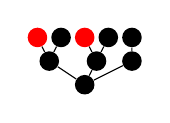
\begin{tikzpicture}[scale=.2]
\node[circle, scale=0.75, fill] (tid0) at (3.75,0){};
\node[circle, scale=0.75, fill] (tid1) at (1.5,1.5){};
\node[circle, scale=0.75, fill, red] (tid4) at (0.75,3){};

\node[circle, scale=0.75, fill] (tid5) at (2.25,3){};

\draw[](tid1) -- (tid4);
\draw[](tid1) -- (tid5);

\node[circle, scale=0.75, fill] (tid2) at (4.5,1.5){};
\node[circle, scale=0.75, fill, red] (tid6) at (3.75,3){};

\node[circle, scale=0.75, fill] (tid7) at (5.25,3){};

\draw[](tid2) -- (tid6);
\draw[](tid2) -- (tid7);

\node[circle, scale=0.75, fill] (tid3) at (6.75,1.5){};
\node[circle, scale=0.75, fill] (tid8) at (6.75,3){};

\draw[](tid3) -- (tid8);

\draw[](tid0) -- (tid1);
\draw[](tid0) -- (tid2);
\draw[](tid0) -- (tid3);

\end{tikzpicture}
};
\node[draw=black] (sn0x9a68588W27) at (27, -30) {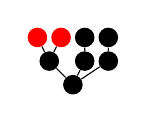
\begin{tikzpicture}[scale=.2]
\node[circle, scale=0.75, fill] (tid0) at (3,0){};
\node[circle, scale=0.75, fill] (tid1) at (1.5,1.5){};
\node[circle, scale=0.75, fill, red] (tid4) at (0.75,3){};

\node[circle, scale=0.75, fill, red] (tid5) at (2.25,3){};

\draw[](tid1) -- (tid4);
\draw[](tid1) -- (tid5);

\node[circle, scale=0.75, fill] (tid2) at (3.75,1.5){};
\node[circle, scale=0.75, fill] (tid6) at (3.75,3){};

\draw[](tid2) -- (tid6);

\node[circle, scale=0.75, fill] (tid3) at (5.25,1.5){};
\node[circle, scale=0.75, fill] (tid7) at (5.25,3){};

\draw[](tid3) -- (tid7);

\draw[](tid0) -- (tid1);
\draw[](tid0) -- (tid2);
\draw[](tid0) -- (tid3);

\end{tikzpicture}
};
\node[draw=black] (sn0x9a6ed08W45) at (45, -40) {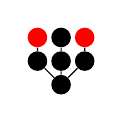
\begin{tikzpicture}[scale=.2]
\node[circle, scale=0.75, fill] (tid0) at (2.25,0){};
\node[circle, scale=0.75, fill] (tid1) at (0.75,1.5){};
\node[circle, scale=0.75, fill, red] (tid4) at (0.75,3){};

\draw[](tid1) -- (tid4);

\node[circle, scale=0.75, fill] (tid2) at (2.25,1.5){};
\node[circle, scale=0.75, fill] (tid5) at (2.25,3){};

\draw[](tid2) -- (tid5);

\node[circle, scale=0.75, fill] (tid3) at (3.75,1.5){};
\node[circle, scale=0.75, fill, red] (tid6) at (3.75,3){};

\draw[](tid3) -- (tid6);

\draw[](tid0) -- (tid1);
\draw[](tid0) -- (tid2);
\draw[](tid0) -- (tid3);

\end{tikzpicture}
};
\draw (sn0x9a6ed08W45.south) -- (sn0x9a6d750W9.north);
\draw (sn0x9a68588W27.south) -- (sn0x9a6cfd8W9.north);
\draw (sn0x9a68588W27.south) -- (sn0x9a6ed08W45.north);
\node[draw=black] (sn0x9a69108W36) at (36, -30) {\begin{tikzpicture}[scale=.2]
\node[circle, scale=0.75, fill] (tid0) at (3,0){};
\node[circle, scale=0.75, fill] (tid1) at (1.5,1.5){};
\node[circle, scale=0.75, fill, red] (tid4) at (0.75,3){};

\node[circle, scale=0.75, fill] (tid5) at (2.25,3){};

\draw[](tid1) -- (tid4);
\draw[](tid1) -- (tid5);

\node[circle, scale=0.75, fill] (tid2) at (3.75,1.5){};
\node[circle, scale=0.75, fill] (tid6) at (3.75,3){};

\draw[](tid2) -- (tid6);

\node[circle, scale=0.75, fill] (tid3) at (5.25,1.5){};
\node[circle, scale=0.75, fill, red] (tid7) at (5.25,3){};

\draw[](tid3) -- (tid7);

\draw[](tid0) -- (tid1);
\draw[](tid0) -- (tid2);
\draw[](tid0) -- (tid3);

\end{tikzpicture}
};
\draw (sn0x9a69108W36.south) -- (sn0x9a6ed08W45.north);
\draw (sn0x9a69108W36.south) -- (sn0x9a6d1a0W18.north);
\draw (sn0x9a69108W36.south) -- (sn0x9a6d4b8W27.north);
\draw (sn0x9a69108W36.south) -- (sn0x9a6d520W36.north);
\draw (sn0x9a68730W18.south) -- (sn0x9a696c8W9.north);
\draw (sn0x9a68730W18.south) -- (sn0x9a68588W27.north);
\draw (sn0x9a68730W18.south) -- (sn0x9a69108W36.north);
\node[draw=black] (sn0x9a707b0W27) at (27, -20) {\begin{tikzpicture}[scale=.2]
\node[circle, scale=0.75, fill] (tid0) at (3.75,0){};
\node[circle, scale=0.75, fill] (tid1) at (1.5,1.5){};
\node[circle, scale=0.75, fill, red] (tid4) at (0.75,3){};

\node[circle, scale=0.75, fill] (tid5) at (2.25,3){};

\draw[](tid1) -- (tid4);
\draw[](tid1) -- (tid5);

\node[circle, scale=0.75, fill] (tid2) at (4.5,1.5){};
\node[circle, scale=0.75, fill] (tid6) at (3.75,3){};

\node[circle, scale=0.75, fill] (tid7) at (5.25,3){};

\draw[](tid2) -- (tid6);
\draw[](tid2) -- (tid7);

\node[circle, scale=0.75, fill] (tid3) at (6.75,1.5){};
\node[circle, scale=0.75, fill, red] (tid8) at (6.75,3){};

\draw[](tid3) -- (tid8);

\draw[](tid0) -- (tid1);
\draw[](tid0) -- (tid2);
\draw[](tid0) -- (tid3);

\end{tikzpicture}
};
\node[draw=black] (sn0x9a70b78W45) at (45, -30) {\begin{tikzpicture}[scale=.2]
\node[circle, scale=0.75, fill] (tid0) at (3.75,0){};
\node[circle, scale=0.75, fill] (tid1) at (1.5,1.5){};
\node[circle, scale=0.75, fill, red] (tid4) at (0.75,3){};

\node[circle, scale=0.75, fill, red] (tid5) at (2.25,3){};

\draw[](tid1) -- (tid4);
\draw[](tid1) -- (tid5);

\node[circle, scale=0.75, fill] (tid2) at (4.5,1.5){};
\node[circle, scale=0.75, fill] (tid6) at (3.75,3){};

\node[circle, scale=0.75, fill] (tid7) at (5.25,3){};

\draw[](tid2) -- (tid6);
\draw[](tid2) -- (tid7);

\node[circle, scale=0.75, fill] (tid3) at (6.75,1.5){};

\draw[](tid0) -- (tid1);
\draw[](tid0) -- (tid2);
\draw[](tid0) -- (tid3);

\end{tikzpicture}
};
\draw (sn0x9a70b78W45.south) -- (sn0x9a6d520W36.north);
\node[draw=black] (sn0x9a6f1b0W54) at (54, -30) {\begin{tikzpicture}[scale=.2]
\node[circle, scale=0.75, fill] (tid0) at (3.75,0){};
\node[circle, scale=0.75, fill] (tid1) at (1.5,1.5){};
\node[circle, scale=0.75, fill, red] (tid4) at (0.75,3){};

\node[circle, scale=0.75, fill] (tid5) at (2.25,3){};

\draw[](tid1) -- (tid4);
\draw[](tid1) -- (tid5);

\node[circle, scale=0.75, fill] (tid2) at (4.5,1.5){};
\node[circle, scale=0.75, fill, red] (tid6) at (3.75,3){};

\node[circle, scale=0.75, fill] (tid7) at (5.25,3){};

\draw[](tid2) -- (tid6);
\draw[](tid2) -- (tid7);

\node[circle, scale=0.75, fill] (tid3) at (6.75,1.5){};

\draw[](tid0) -- (tid1);
\draw[](tid0) -- (tid2);
\draw[](tid0) -- (tid3);

\end{tikzpicture}
};
\draw (sn0x9a6f1b0W54.south) -- (sn0x9a6d520W36.north);
\draw (sn0x9a6f1b0W54.south) -- (sn0x9a6d4b8W27.north);
\draw (sn0x9a707b0W27.south) -- (sn0x9a6ef58W18.north);
\draw (sn0x9a707b0W27.south) -- (sn0x9a69108W36.north);
\draw (sn0x9a707b0W27.south) -- (sn0x9a70b78W45.north);
\draw (sn0x9a707b0W27.south) -- (sn0x9a6f1b0W54.north);
\draw (sn0x9a689f0W9.south) -- (sn0x9a70650W9.north);
\draw (sn0x9a689f0W9.south) -- (sn0x9a68730W18.north);
\draw (sn0x9a689f0W9.south) -- (sn0x9a707b0W27.north);
\end{tikzpicture}

%%% Local Variables:
%%% TeX-master: "thesis/thesis.tex"
%%% End: 

\begin{tikzpicture}[scale=.2, anchor=base]
\node[draw=black] (sn0x9a68a50W9) at (9, -10) {\begin{tikzpicture}[scale=.2]
\node[circle, scale=0.75, fill] (tid0) at (4.5,0){};
\node[circle, scale=0.75, fill] (tid1) at (2.25,1.5){};
\node[circle, scale=0.75, fill, red] (tid4) at (0.75,3){};

\node[circle, scale=0.75, fill] (tid5) at (2.25,3){};

\node[circle, scale=0.75, fill] (tid6) at (3.75,3){};

\draw[](tid1) -- (tid4);
\draw[](tid1) -- (tid5);
\draw[](tid1) -- (tid6);

\node[circle, scale=0.75, fill] (tid2) at (6,1.5){};
\node[circle, scale=0.75, fill] (tid7) at (5.25,3){};

\node[circle, scale=0.75, fill] (tid8) at (6.75,3){};

\draw[](tid2) -- (tid7);
\draw[](tid2) -- (tid8);

\node[circle, scale=0.75, fill] (tid3) at (8.25,1.5){};
\node[circle, scale=0.75, fill, red] (tid9) at (8.25,3){};

\draw[](tid3) -- (tid9);

\draw[](tid0) -- (tid1);
\draw[](tid0) -- (tid2);
\draw[](tid0) -- (tid3);

\end{tikzpicture}
};
\node[draw=black] (sn0x9a707b0W9) at (9, -20) {\begin{tikzpicture}[scale=.2]
\node[circle, scale=0.75, fill] (tid0) at (3.75,0){};
\node[circle, scale=0.75, fill] (tid1) at (1.5,1.5){};
\node[circle, scale=0.75, fill, red] (tid4) at (0.75,3){};

\node[circle, scale=0.75, fill] (tid5) at (2.25,3){};

\draw[](tid1) -- (tid4);
\draw[](tid1) -- (tid5);

\node[circle, scale=0.75, fill] (tid2) at (4.5,1.5){};
\node[circle, scale=0.75, fill] (tid6) at (3.75,3){};

\node[circle, scale=0.75, fill] (tid7) at (5.25,3){};

\draw[](tid2) -- (tid6);
\draw[](tid2) -- (tid7);

\node[circle, scale=0.75, fill] (tid3) at (6.75,1.5){};
\node[circle, scale=0.75, fill, red] (tid8) at (6.75,3){};

\draw[](tid3) -- (tid8);

\draw[](tid0) -- (tid1);
\draw[](tid0) -- (tid2);
\draw[](tid0) -- (tid3);

\end{tikzpicture}
};
\node[draw=black] (sn0x9a6ef58W9) at (9, -30) {\begin{tikzpicture}[scale=.2]
\node[circle, scale=0.75, fill] (tid0) at (3,0){};
\node[circle, scale=0.75, fill] (tid1) at (1.5,1.5){};
\node[circle, scale=0.75, fill] (tid4) at (0.75,3){};

\node[circle, scale=0.75, fill] (tid5) at (2.25,3){};

\draw[](tid1) -- (tid4);
\draw[](tid1) -- (tid5);

\node[circle, scale=0.75, fill] (tid2) at (3.75,1.5){};
\node[circle, scale=0.75, fill, red] (tid6) at (3.75,3){};

\draw[](tid2) -- (tid6);

\node[circle, scale=0.75, fill] (tid3) at (5.25,1.5){};
\node[circle, scale=0.75, fill, red] (tid7) at (5.25,3){};

\draw[](tid3) -- (tid7);

\draw[](tid0) -- (tid1);
\draw[](tid0) -- (tid2);
\draw[](tid0) -- (tid3);

\end{tikzpicture}
};
\node[draw=black] (sn0x9a6d520W9) at (9, -40) {\begin{tikzpicture}[scale=.2]
\node[circle, scale=0.75, fill] (tid0) at (3,0){};
\node[circle, scale=0.75, fill] (tid1) at (1.5,1.5){};
\node[circle, scale=0.75, fill, red] (tid4) at (0.75,3){};

\node[circle, scale=0.75, fill] (tid5) at (2.25,3){};

\draw[](tid1) -- (tid4);
\draw[](tid1) -- (tid5);

\node[circle, scale=0.75, fill] (tid2) at (3.75,1.5){};
\node[circle, scale=0.75, fill, red] (tid6) at (3.75,3){};

\draw[](tid2) -- (tid6);

\node[circle, scale=0.75, fill] (tid3) at (5.25,1.5){};

\draw[](tid0) -- (tid1);
\draw[](tid0) -- (tid2);
\draw[](tid0) -- (tid3);

\end{tikzpicture}
};
\node[draw=black] (sn0x9a6d750W9) at (9, -50) {\begin{tikzpicture}[scale=.2]
\node[circle, scale=0.75, fill] (tid0) at (2.25,0){};
\node[circle, scale=0.75, fill] (tid1) at (0.75,1.5){};
\node[circle, scale=0.75, fill, red] (tid4) at (0.75,3){};

\draw[](tid1) -- (tid4);

\node[circle, scale=0.75, fill] (tid2) at (2.25,1.5){};
\node[circle, scale=0.75, fill, red] (tid5) at (2.25,3){};

\draw[](tid2) -- (tid5);

\node[circle, scale=0.75, fill] (tid3) at (3.75,1.5){};

\draw[](tid0) -- (tid1);
\draw[](tid0) -- (tid2);
\draw[](tid0) -- (tid3);

\end{tikzpicture}
};
\node[draw=black] (sn0x9a6da10W9) at (9, -60) {\begin{tikzpicture}[scale=.2]
\node[circle, scale=0.75, fill] (tid0) at (2.25,0){};
\node[circle, scale=0.75, fill] (tid1) at (0.75,1.5){};
\node[circle, scale=0.75, fill, red] (tid4) at (0.75,3){};

\draw[](tid1) -- (tid4);

\node[circle, scale=0.75, fill, red] (tid2) at (2.25,1.5){};

\node[circle, scale=0.75, fill] (tid3) at (3.75,1.5){};

\draw[](tid0) -- (tid1);
\draw[](tid0) -- (tid2);
\draw[](tid0) -- (tid3);

\end{tikzpicture}
};
\node[draw=black] (sn0x9a6d990W9) at (9, -70) {\begin{tikzpicture}[scale=.2]
\node[circle, scale=0.75, fill] (tid0) at (1.5,0){};
\node[circle, scale=0.75, fill] (tid1) at (0.75,1.5){};
\node[circle, scale=0.75, fill, red] (tid3) at (0.75,3){};

\draw[](tid1) -- (tid3);

\node[circle, scale=0.75, fill, red] (tid2) at (2.25,1.5){};

\draw[](tid0) -- (tid1);
\draw[](tid0) -- (tid2);

\end{tikzpicture}
};
\node[draw=black] (sn0x9a6dd40W9) at (9, -80) {\begin{tikzpicture}[scale=.2]
\node[circle, scale=0.75, fill] (tid0) at (0.75,0){};
\node[circle, scale=0.75, fill] (tid1) at (0.75,1.5){};
\node[circle, scale=0.75, fill, red] (tid2) at (0.75,3){};

\draw[](tid1) -- (tid2);

\draw[](tid0) -- (tid1);

\end{tikzpicture}
};
\node[draw=black] (sn0x9a6e148W9) at (9, -90) {\begin{tikzpicture}[scale=.2]
\node[circle, scale=0.75, fill] (tid0) at (0.75,0){};
\node[circle, scale=0.75, fill, red] (tid1) at (0.75,1.5){};

\draw[](tid0) -- (tid1);

\end{tikzpicture}
};
\node[draw=black] (sn0x9a6e1b0W9) at (9, -100) {\begin{tikzpicture}[scale=.2]
\node[circle, scale=0.75, fill] (tid0) at (0.75,0){};

\end{tikzpicture}
};
\draw (sn0x9a6e148W9.south) -- (sn0x9a6e1b0W9.north);
\draw (sn0x9a6dd40W9.south) -- (sn0x9a6e148W9.north);
\node[draw=black] (sn0x9a6dff8W18) at (18, -80) {\begin{tikzpicture}[scale=.2]
\node[circle, scale=0.75, fill] (tid0) at (1.5,0){};
\node[circle, scale=0.75, fill, red] (tid1) at (0.75,1.5){};

\node[circle, scale=0.75, fill, red] (tid2) at (2.25,1.5){};

\draw[](tid0) -- (tid1);
\draw[](tid0) -- (tid2);

\end{tikzpicture}
};
\draw (sn0x9a6dff8W18.south) -- (sn0x9a6e148W9.north);
\draw (sn0x9a6d990W9.south) -- (sn0x9a6dd40W9.north);
\draw (sn0x9a6d990W9.south) -- (sn0x9a6dff8W18.north);
\node[draw=black] (sn0x9a6dcd8W18) at (18, -70) {\begin{tikzpicture}[scale=.2]
\node[circle, scale=0.75, fill] (tid0) at (2.25,0){};
\node[circle, scale=0.75, fill, red] (tid1) at (0.75,1.5){};

\node[circle, scale=0.75, fill, red] (tid2) at (2.25,1.5){};

\node[circle, scale=0.75, fill] (tid3) at (3.75,1.5){};

\draw[](tid0) -- (tid1);
\draw[](tid0) -- (tid2);
\draw[](tid0) -- (tid3);

\end{tikzpicture}
};
\draw (sn0x9a6dcd8W18.south) -- (sn0x9a6dff8W18.north);
\draw (sn0x9a6da10W9.south) -- (sn0x9a6d990W9.north);
\draw (sn0x9a6da10W9.south) -- (sn0x9a6dcd8W18.north);
\draw (sn0x9a6d750W9.south) -- (sn0x9a6da10W9.north);
\node[draw=black] (sn0x9a6e378W18) at (18, -50) {\begin{tikzpicture}[scale=.2]
\node[circle, scale=0.75, fill] (tid0) at (3,0){};
\node[circle, scale=0.75, fill] (tid1) at (1.5,1.5){};
\node[circle, scale=0.75, fill, red] (tid4) at (0.75,3){};

\node[circle, scale=0.75, fill, red] (tid5) at (2.25,3){};

\draw[](tid1) -- (tid4);
\draw[](tid1) -- (tid5);

\node[circle, scale=0.75, fill] (tid2) at (3.75,1.5){};

\node[circle, scale=0.75, fill] (tid3) at (5.25,1.5){};

\draw[](tid0) -- (tid1);
\draw[](tid0) -- (tid2);
\draw[](tid0) -- (tid3);

\end{tikzpicture}
};
\draw (sn0x9a6e378W18.south) -- (sn0x9a6da10W9.north);
\draw (sn0x9a6d520W9.south) -- (sn0x9a6d750W9.north);
\draw (sn0x9a6d520W9.south) -- (sn0x9a6e378W18.north);
\draw (sn0x9a6ef58W9.south) -- (sn0x9a6d520W9.north);
\node[draw=black] (sn0x9a69108W18) at (18, -30) {\begin{tikzpicture}[scale=.2]
\node[circle, scale=0.75, fill] (tid0) at (3,0){};
\node[circle, scale=0.75, fill] (tid1) at (1.5,1.5){};
\node[circle, scale=0.75, fill, red] (tid4) at (0.75,3){};

\node[circle, scale=0.75, fill] (tid5) at (2.25,3){};

\draw[](tid1) -- (tid4);
\draw[](tid1) -- (tid5);

\node[circle, scale=0.75, fill] (tid2) at (3.75,1.5){};
\node[circle, scale=0.75, fill] (tid6) at (3.75,3){};

\draw[](tid2) -- (tid6);

\node[circle, scale=0.75, fill] (tid3) at (5.25,1.5){};
\node[circle, scale=0.75, fill, red] (tid7) at (5.25,3){};

\draw[](tid3) -- (tid7);

\draw[](tid0) -- (tid1);
\draw[](tid0) -- (tid2);
\draw[](tid0) -- (tid3);

\end{tikzpicture}
};
\node[draw=black] (sn0x9a6ed08W18) at (18, -40) {\begin{tikzpicture}[scale=.2]
\node[circle, scale=0.75, fill] (tid0) at (2.25,0){};
\node[circle, scale=0.75, fill] (tid1) at (0.75,1.5){};
\node[circle, scale=0.75, fill, red] (tid4) at (0.75,3){};

\draw[](tid1) -- (tid4);

\node[circle, scale=0.75, fill] (tid2) at (2.25,1.5){};
\node[circle, scale=0.75, fill] (tid5) at (2.25,3){};

\draw[](tid2) -- (tid5);

\node[circle, scale=0.75, fill] (tid3) at (3.75,1.5){};
\node[circle, scale=0.75, fill, red] (tid6) at (3.75,3){};

\draw[](tid3) -- (tid6);

\draw[](tid0) -- (tid1);
\draw[](tid0) -- (tid2);
\draw[](tid0) -- (tid3);

\end{tikzpicture}
};
\draw (sn0x9a6ed08W18.south) -- (sn0x9a6d750W9.north);
\node[draw=black] (sn0x9a6d1a0W27) at (27, -40) {\begin{tikzpicture}[scale=.2]
\node[circle, scale=0.75, fill] (tid0) at (2.25,0){};
\node[circle, scale=0.75, fill] (tid1) at (0.75,1.5){};
\node[circle, scale=0.75, fill] (tid4) at (0.75,3){};

\draw[](tid1) -- (tid4);

\node[circle, scale=0.75, fill] (tid2) at (2.25,1.5){};
\node[circle, scale=0.75, fill, red] (tid5) at (2.25,3){};

\draw[](tid2) -- (tid5);

\node[circle, scale=0.75, fill] (tid3) at (3.75,1.5){};
\node[circle, scale=0.75, fill, red] (tid6) at (3.75,3){};

\draw[](tid3) -- (tid6);

\draw[](tid0) -- (tid1);
\draw[](tid0) -- (tid2);
\draw[](tid0) -- (tid3);

\end{tikzpicture}
};
\draw (sn0x9a6d1a0W27.south) -- (sn0x9a6d750W9.north);
\node[draw=black] (sn0x9a6d4b8W36) at (36, -40) {\begin{tikzpicture}[scale=.2]
\node[circle, scale=0.75, fill] (tid0) at (3,0){};
\node[circle, scale=0.75, fill] (tid1) at (1.5,1.5){};
\node[circle, scale=0.75, fill, red] (tid4) at (0.75,3){};

\node[circle, scale=0.75, fill, red] (tid5) at (2.25,3){};

\draw[](tid1) -- (tid4);
\draw[](tid1) -- (tid5);

\node[circle, scale=0.75, fill] (tid2) at (3.75,1.5){};
\node[circle, scale=0.75, fill] (tid6) at (3.75,3){};

\draw[](tid2) -- (tid6);

\node[circle, scale=0.75, fill] (tid3) at (5.25,1.5){};

\draw[](tid0) -- (tid1);
\draw[](tid0) -- (tid2);
\draw[](tid0) -- (tid3);

\end{tikzpicture}
};
\draw (sn0x9a6d4b8W36.south) -- (sn0x9a6d750W9.north);
\draw (sn0x9a69108W18.south) -- (sn0x9a6ed08W18.north);
\draw (sn0x9a69108W18.south) -- (sn0x9a6d1a0W27.north);
\draw (sn0x9a69108W18.south) -- (sn0x9a6d4b8W36.north);
\draw (sn0x9a69108W18.south) -- (sn0x9a6d520W9.north);
\node[draw=black] (sn0x9a70b78W27) at (27, -30) {\begin{tikzpicture}[scale=.2]
\node[circle, scale=0.75, fill] (tid0) at (3.75,0){};
\node[circle, scale=0.75, fill] (tid1) at (1.5,1.5){};
\node[circle, scale=0.75, fill, red] (tid4) at (0.75,3){};

\node[circle, scale=0.75, fill, red] (tid5) at (2.25,3){};

\draw[](tid1) -- (tid4);
\draw[](tid1) -- (tid5);

\node[circle, scale=0.75, fill] (tid2) at (4.5,1.5){};
\node[circle, scale=0.75, fill] (tid6) at (3.75,3){};

\node[circle, scale=0.75, fill] (tid7) at (5.25,3){};

\draw[](tid2) -- (tid6);
\draw[](tid2) -- (tid7);

\node[circle, scale=0.75, fill] (tid3) at (6.75,1.5){};

\draw[](tid0) -- (tid1);
\draw[](tid0) -- (tid2);
\draw[](tid0) -- (tid3);

\end{tikzpicture}
};
\draw (sn0x9a70b78W27.south) -- (sn0x9a6d520W9.north);
\node[draw=black] (sn0x9a6f1b0W36) at (36, -30) {\begin{tikzpicture}[scale=.2]
\node[circle, scale=0.75, fill] (tid0) at (3.75,0){};
\node[circle, scale=0.75, fill] (tid1) at (1.5,1.5){};
\node[circle, scale=0.75, fill, red] (tid4) at (0.75,3){};

\node[circle, scale=0.75, fill] (tid5) at (2.25,3){};

\draw[](tid1) -- (tid4);
\draw[](tid1) -- (tid5);

\node[circle, scale=0.75, fill] (tid2) at (4.5,1.5){};
\node[circle, scale=0.75, fill, red] (tid6) at (3.75,3){};

\node[circle, scale=0.75, fill] (tid7) at (5.25,3){};

\draw[](tid2) -- (tid6);
\draw[](tid2) -- (tid7);

\node[circle, scale=0.75, fill] (tid3) at (6.75,1.5){};

\draw[](tid0) -- (tid1);
\draw[](tid0) -- (tid2);
\draw[](tid0) -- (tid3);

\end{tikzpicture}
};
\draw (sn0x9a6f1b0W36.south) -- (sn0x9a6d520W9.north);
\draw (sn0x9a6f1b0W36.south) -- (sn0x9a6d4b8W36.north);
\draw (sn0x9a707b0W9.south) -- (sn0x9a6ef58W9.north);
\draw (sn0x9a707b0W9.south) -- (sn0x9a69108W18.north);
\draw (sn0x9a707b0W9.south) -- (sn0x9a70b78W27.north);
\draw (sn0x9a707b0W9.south) -- (sn0x9a6f1b0W36.north);
\node[draw=black] (sn0x9a69cd8W18) at (18, -20) {\begin{tikzpicture}[scale=.2]
\node[circle, scale=0.75, fill] (tid0) at (3.75,0){};
\node[circle, scale=0.75, fill] (tid1) at (1.5,1.5){};
\node[circle, scale=0.75, fill] (tid4) at (0.75,3){};

\node[circle, scale=0.75, fill] (tid5) at (2.25,3){};

\draw[](tid1) -- (tid4);
\draw[](tid1) -- (tid5);

\node[circle, scale=0.75, fill] (tid2) at (4.5,1.5){};
\node[circle, scale=0.75, fill, red] (tid6) at (3.75,3){};

\node[circle, scale=0.75, fill] (tid7) at (5.25,3){};

\draw[](tid2) -- (tid6);
\draw[](tid2) -- (tid7);

\node[circle, scale=0.75, fill] (tid3) at (6.75,1.5){};
\node[circle, scale=0.75, fill, red] (tid8) at (6.75,3){};

\draw[](tid3) -- (tid8);

\draw[](tid0) -- (tid1);
\draw[](tid0) -- (tid2);
\draw[](tid0) -- (tid3);

\end{tikzpicture}
};
\node[draw=black] (sn0x9a6f4c0W45) at (45, -30) {\begin{tikzpicture}[scale=.2]
\node[circle, scale=0.75, fill] (tid0) at (3.75,0){};
\node[circle, scale=0.75, fill] (tid1) at (1.5,1.5){};
\node[circle, scale=0.75, fill] (tid4) at (0.75,3){};

\node[circle, scale=0.75, fill] (tid5) at (2.25,3){};

\draw[](tid1) -- (tid4);
\draw[](tid1) -- (tid5);

\node[circle, scale=0.75, fill] (tid2) at (4.5,1.5){};
\node[circle, scale=0.75, fill, red] (tid6) at (3.75,3){};

\node[circle, scale=0.75, fill, red] (tid7) at (5.25,3){};

\draw[](tid2) -- (tid6);
\draw[](tid2) -- (tid7);

\node[circle, scale=0.75, fill] (tid3) at (6.75,1.5){};

\draw[](tid0) -- (tid1);
\draw[](tid0) -- (tid2);
\draw[](tid0) -- (tid3);

\end{tikzpicture}
};
\draw (sn0x9a6f4c0W45.south) -- (sn0x9a6d520W9.north);
\draw (sn0x9a69cd8W18.south) -- (sn0x9a69108W18.north);
\draw (sn0x9a69cd8W18.south) -- (sn0x9a6ef58W9.north);
\draw (sn0x9a69cd8W18.south) -- (sn0x9a6f1b0W36.north);
\draw (sn0x9a69cd8W18.south) -- (sn0x9a6f4c0W45.north);
\node[draw=black] (sn0x9a70df0W27) at (27, -20) {\begin{tikzpicture}[scale=.2]
\node[circle, scale=0.75, fill] (tid0) at (4.5,0){};
\node[circle, scale=0.75, fill] (tid1) at (2.25,1.5){};
\node[circle, scale=0.75, fill, red] (tid4) at (0.75,3){};

\node[circle, scale=0.75, fill, red] (tid5) at (2.25,3){};

\node[circle, scale=0.75, fill] (tid6) at (3.75,3){};

\draw[](tid1) -- (tid4);
\draw[](tid1) -- (tid5);
\draw[](tid1) -- (tid6);

\node[circle, scale=0.75, fill] (tid2) at (6,1.5){};
\node[circle, scale=0.75, fill] (tid7) at (5.25,3){};

\node[circle, scale=0.75, fill] (tid8) at (6.75,3){};

\draw[](tid2) -- (tid7);
\draw[](tid2) -- (tid8);

\node[circle, scale=0.75, fill] (tid3) at (8.25,1.5){};

\draw[](tid0) -- (tid1);
\draw[](tid0) -- (tid2);
\draw[](tid0) -- (tid3);

\end{tikzpicture}
};
\draw (sn0x9a70df0W27.south) -- (sn0x9a70b78W27.north);
\draw (sn0x9a70df0W27.south) -- (sn0x9a6f1b0W36.north);
\node[draw=black] (sn0x9a71218W36) at (36, -20) {\begin{tikzpicture}[scale=.2]
\node[circle, scale=0.75, fill] (tid0) at (4.5,0){};
\node[circle, scale=0.75, fill] (tid1) at (2.25,1.5){};
\node[circle, scale=0.75, fill, red] (tid4) at (0.75,3){};

\node[circle, scale=0.75, fill] (tid5) at (2.25,3){};

\node[circle, scale=0.75, fill] (tid6) at (3.75,3){};

\draw[](tid1) -- (tid4);
\draw[](tid1) -- (tid5);
\draw[](tid1) -- (tid6);

\node[circle, scale=0.75, fill] (tid2) at (6,1.5){};
\node[circle, scale=0.75, fill, red] (tid7) at (5.25,3){};

\node[circle, scale=0.75, fill] (tid8) at (6.75,3){};

\draw[](tid2) -- (tid7);
\draw[](tid2) -- (tid8);

\node[circle, scale=0.75, fill] (tid3) at (8.25,1.5){};

\draw[](tid0) -- (tid1);
\draw[](tid0) -- (tid2);
\draw[](tid0) -- (tid3);

\end{tikzpicture}
};
\node[draw=black] (sn0x9a6f8b0W54) at (54, -30) {\begin{tikzpicture}[scale=.2]
\node[circle, scale=0.75, fill] (tid0) at (3.75,0){};
\node[circle, scale=0.75, fill] (tid1) at (2.25,1.5){};
\node[circle, scale=0.75, fill, red] (tid4) at (0.75,3){};

\node[circle, scale=0.75, fill, red] (tid5) at (2.25,3){};

\node[circle, scale=0.75, fill] (tid6) at (3.75,3){};

\draw[](tid1) -- (tid4);
\draw[](tid1) -- (tid5);
\draw[](tid1) -- (tid6);

\node[circle, scale=0.75, fill] (tid2) at (5.25,1.5){};
\node[circle, scale=0.75, fill] (tid7) at (5.25,3){};

\draw[](tid2) -- (tid7);

\node[circle, scale=0.75, fill] (tid3) at (6.75,1.5){};

\draw[](tid0) -- (tid1);
\draw[](tid0) -- (tid2);
\draw[](tid0) -- (tid3);

\end{tikzpicture}
};
\draw (sn0x9a6f8b0W54.south) -- (sn0x9a6d4b8W36.north);
\draw (sn0x9a6f8b0W54.south) -- (sn0x9a6d520W9.north);
\node[draw=black] (sn0x9a6fc50W63) at (63, -30) {\begin{tikzpicture}[scale=.2]
\node[circle, scale=0.75, fill] (tid0) at (3.75,0){};
\node[circle, scale=0.75, fill] (tid1) at (2.25,1.5){};
\node[circle, scale=0.75, fill, red] (tid4) at (0.75,3){};

\node[circle, scale=0.75, fill] (tid5) at (2.25,3){};

\node[circle, scale=0.75, fill] (tid6) at (3.75,3){};

\draw[](tid1) -- (tid4);
\draw[](tid1) -- (tid5);
\draw[](tid1) -- (tid6);

\node[circle, scale=0.75, fill] (tid2) at (5.25,1.5){};
\node[circle, scale=0.75, fill, red] (tid7) at (5.25,3){};

\draw[](tid2) -- (tid7);

\node[circle, scale=0.75, fill] (tid3) at (6.75,1.5){};

\draw[](tid0) -- (tid1);
\draw[](tid0) -- (tid2);
\draw[](tid0) -- (tid3);

\end{tikzpicture}
};
\node[draw=black] (sn0x9a6fe48W45) at (45, -40) {\begin{tikzpicture}[scale=.2]
\node[circle, scale=0.75, fill] (tid0) at (3.75,0){};
\node[circle, scale=0.75, fill] (tid1) at (2.25,1.5){};
\node[circle, scale=0.75, fill, red] (tid4) at (0.75,3){};

\node[circle, scale=0.75, fill, red] (tid5) at (2.25,3){};

\node[circle, scale=0.75, fill] (tid6) at (3.75,3){};

\draw[](tid1) -- (tid4);
\draw[](tid1) -- (tid5);
\draw[](tid1) -- (tid6);

\node[circle, scale=0.75, fill] (tid2) at (5.25,1.5){};

\node[circle, scale=0.75, fill] (tid3) at (6.75,1.5){};

\draw[](tid0) -- (tid1);
\draw[](tid0) -- (tid2);
\draw[](tid0) -- (tid3);

\end{tikzpicture}
};
\draw (sn0x9a6fe48W45.south) -- (sn0x9a6e378W18.north);
\draw (sn0x9a6fc50W63.south) -- (sn0x9a6d520W9.north);
\draw (sn0x9a6fc50W63.south) -- (sn0x9a6fe48W45.north);
\draw (sn0x9a71218W36.south) -- (sn0x9a6f1b0W36.north);
\draw (sn0x9a71218W36.south) -- (sn0x9a6f4c0W45.north);
\draw (sn0x9a71218W36.south) -- (sn0x9a6f8b0W54.north);
\draw (sn0x9a71218W36.south) -- (sn0x9a6fc50W63.north);
\draw (sn0x9a68a50W9.south) -- (sn0x9a707b0W9.north);
\draw (sn0x9a68a50W9.south) -- (sn0x9a69cd8W18.north);
\draw (sn0x9a68a50W9.south) -- (sn0x9a70df0W27.north);
\draw (sn0x9a68a50W9.south) -- (sn0x9a71218W36.north);
\end{tikzpicture}

%%% Local Variables:
%%% TeX-master: "thesis/thesis.tex"
%%% End: 

\begin{tikzpicture}[scale=.2, anchor=base]
\node[draw=black] (sn0x9a68ab0W9) at (9, -10) {\begin{tikzpicture}[scale=.2]
\node[circle, scale=0.75, fill] (tid0) at (4.5,0){};
\node[circle, scale=0.75, fill] (tid1) at (2.25,1.5){};
\node[circle, scale=0.75, fill] (tid4) at (0.75,3){};

\node[circle, scale=0.75, fill] (tid5) at (2.25,3){};

\node[circle, scale=0.75, fill] (tid6) at (3.75,3){};

\draw[](tid1) -- (tid4);
\draw[](tid1) -- (tid5);
\draw[](tid1) -- (tid6);

\node[circle, scale=0.75, fill] (tid2) at (6,1.5){};
\node[circle, scale=0.75, fill, red] (tid7) at (5.25,3){};

\node[circle, scale=0.75, fill, red] (tid8) at (6.75,3){};

\draw[](tid2) -- (tid7);
\draw[](tid2) -- (tid8);

\node[circle, scale=0.75, fill] (tid3) at (8.25,1.5){};
\node[circle, scale=0.75, fill] (tid9) at (8.25,3){};

\draw[](tid3) -- (tid9);

\draw[](tid0) -- (tid1);
\draw[](tid0) -- (tid2);
\draw[](tid0) -- (tid3);

\end{tikzpicture}
};
\node[draw=black] (sn0x9a697e0W9) at (9, -20) {\begin{tikzpicture}[scale=.2]
\node[circle, scale=0.75, fill] (tid0) at (3.75,0){};
\node[circle, scale=0.75, fill] (tid1) at (2.25,1.5){};
\node[circle, scale=0.75, fill, red] (tid4) at (0.75,3){};

\node[circle, scale=0.75, fill] (tid5) at (2.25,3){};

\node[circle, scale=0.75, fill] (tid6) at (3.75,3){};

\draw[](tid1) -- (tid4);
\draw[](tid1) -- (tid5);
\draw[](tid1) -- (tid6);

\node[circle, scale=0.75, fill] (tid2) at (5.25,1.5){};
\node[circle, scale=0.75, fill, red] (tid7) at (5.25,3){};

\draw[](tid2) -- (tid7);

\node[circle, scale=0.75, fill] (tid3) at (6.75,1.5){};
\node[circle, scale=0.75, fill] (tid8) at (6.75,3){};

\draw[](tid3) -- (tid8);

\draw[](tid0) -- (tid1);
\draw[](tid0) -- (tid2);
\draw[](tid0) -- (tid3);

\end{tikzpicture}
};
\node[draw=black] (sn0x9a696c8W9) at (9, -30) {\begin{tikzpicture}[scale=.2]
\node[circle, scale=0.75, fill] (tid0) at (3,0){};
\node[circle, scale=0.75, fill] (tid1) at (1.5,1.5){};
\node[circle, scale=0.75, fill, red] (tid4) at (0.75,3){};

\node[circle, scale=0.75, fill] (tid5) at (2.25,3){};

\draw[](tid1) -- (tid4);
\draw[](tid1) -- (tid5);

\node[circle, scale=0.75, fill] (tid2) at (3.75,1.5){};
\node[circle, scale=0.75, fill, red] (tid6) at (3.75,3){};

\draw[](tid2) -- (tid6);

\node[circle, scale=0.75, fill] (tid3) at (5.25,1.5){};
\node[circle, scale=0.75, fill] (tid7) at (5.25,3){};

\draw[](tid3) -- (tid7);

\draw[](tid0) -- (tid1);
\draw[](tid0) -- (tid2);
\draw[](tid0) -- (tid3);

\end{tikzpicture}
};
\node[draw=black] (sn0x9a6cfd8W9) at (9, -40) {\begin{tikzpicture}[scale=.2]
\node[circle, scale=0.75, fill] (tid0) at (2.25,0){};
\node[circle, scale=0.75, fill] (tid1) at (0.75,1.5){};
\node[circle, scale=0.75, fill, red] (tid4) at (0.75,3){};

\draw[](tid1) -- (tid4);

\node[circle, scale=0.75, fill] (tid2) at (2.25,1.5){};
\node[circle, scale=0.75, fill, red] (tid5) at (2.25,3){};

\draw[](tid2) -- (tid5);

\node[circle, scale=0.75, fill] (tid3) at (3.75,1.5){};
\node[circle, scale=0.75, fill] (tid6) at (3.75,3){};

\draw[](tid3) -- (tid6);

\draw[](tid0) -- (tid1);
\draw[](tid0) -- (tid2);
\draw[](tid0) -- (tid3);

\end{tikzpicture}
};
\node[draw=black] (sn0x9a6d750W9) at (9, -50) {\begin{tikzpicture}[scale=.2]
\node[circle, scale=0.75, fill] (tid0) at (2.25,0){};
\node[circle, scale=0.75, fill] (tid1) at (0.75,1.5){};
\node[circle, scale=0.75, fill, red] (tid4) at (0.75,3){};

\draw[](tid1) -- (tid4);

\node[circle, scale=0.75, fill] (tid2) at (2.25,1.5){};
\node[circle, scale=0.75, fill, red] (tid5) at (2.25,3){};

\draw[](tid2) -- (tid5);

\node[circle, scale=0.75, fill] (tid3) at (3.75,1.5){};

\draw[](tid0) -- (tid1);
\draw[](tid0) -- (tid2);
\draw[](tid0) -- (tid3);

\end{tikzpicture}
};
\node[draw=black] (sn0x9a6da10W9) at (9, -60) {\begin{tikzpicture}[scale=.2]
\node[circle, scale=0.75, fill] (tid0) at (2.25,0){};
\node[circle, scale=0.75, fill] (tid1) at (0.75,1.5){};
\node[circle, scale=0.75, fill, red] (tid4) at (0.75,3){};

\draw[](tid1) -- (tid4);

\node[circle, scale=0.75, fill, red] (tid2) at (2.25,1.5){};

\node[circle, scale=0.75, fill] (tid3) at (3.75,1.5){};

\draw[](tid0) -- (tid1);
\draw[](tid0) -- (tid2);
\draw[](tid0) -- (tid3);

\end{tikzpicture}
};
\node[draw=black] (sn0x9a6d990W9) at (9, -70) {\begin{tikzpicture}[scale=.2]
\node[circle, scale=0.75, fill] (tid0) at (1.5,0){};
\node[circle, scale=0.75, fill] (tid1) at (0.75,1.5){};
\node[circle, scale=0.75, fill, red] (tid3) at (0.75,3){};

\draw[](tid1) -- (tid3);

\node[circle, scale=0.75, fill, red] (tid2) at (2.25,1.5){};

\draw[](tid0) -- (tid1);
\draw[](tid0) -- (tid2);

\end{tikzpicture}
};
\node[draw=black] (sn0x9a6dd40W9) at (9, -80) {\begin{tikzpicture}[scale=.2]
\node[circle, scale=0.75, fill] (tid0) at (0.75,0){};
\node[circle, scale=0.75, fill] (tid1) at (0.75,1.5){};
\node[circle, scale=0.75, fill, red] (tid2) at (0.75,3){};

\draw[](tid1) -- (tid2);

\draw[](tid0) -- (tid1);

\end{tikzpicture}
};
\node[draw=black] (sn0x9a6e148W9) at (9, -90) {\begin{tikzpicture}[scale=.2]
\node[circle, scale=0.75, fill] (tid0) at (0.75,0){};
\node[circle, scale=0.75, fill, red] (tid1) at (0.75,1.5){};

\draw[](tid0) -- (tid1);

\end{tikzpicture}
};
\node[draw=black] (sn0x9a6e1b0W9) at (9, -100) {\begin{tikzpicture}[scale=.2]
\node[circle, scale=0.75, fill] (tid0) at (0.75,0){};

\end{tikzpicture}
};
\draw (sn0x9a6e148W9.south) -- (sn0x9a6e1b0W9.north);
\draw (sn0x9a6dd40W9.south) -- (sn0x9a6e148W9.north);
\node[draw=black] (sn0x9a6dff8W18) at (18, -80) {\begin{tikzpicture}[scale=.2]
\node[circle, scale=0.75, fill] (tid0) at (1.5,0){};
\node[circle, scale=0.75, fill, red] (tid1) at (0.75,1.5){};

\node[circle, scale=0.75, fill, red] (tid2) at (2.25,1.5){};

\draw[](tid0) -- (tid1);
\draw[](tid0) -- (tid2);

\end{tikzpicture}
};
\draw (sn0x9a6dff8W18.south) -- (sn0x9a6e148W9.north);
\draw (sn0x9a6d990W9.south) -- (sn0x9a6dd40W9.north);
\draw (sn0x9a6d990W9.south) -- (sn0x9a6dff8W18.north);
\node[draw=black] (sn0x9a6dcd8W18) at (18, -70) {\begin{tikzpicture}[scale=.2]
\node[circle, scale=0.75, fill] (tid0) at (2.25,0){};
\node[circle, scale=0.75, fill, red] (tid1) at (0.75,1.5){};

\node[circle, scale=0.75, fill, red] (tid2) at (2.25,1.5){};

\node[circle, scale=0.75, fill] (tid3) at (3.75,1.5){};

\draw[](tid0) -- (tid1);
\draw[](tid0) -- (tid2);
\draw[](tid0) -- (tid3);

\end{tikzpicture}
};
\draw (sn0x9a6dcd8W18.south) -- (sn0x9a6dff8W18.north);
\draw (sn0x9a6da10W9.south) -- (sn0x9a6d990W9.north);
\draw (sn0x9a6da10W9.south) -- (sn0x9a6dcd8W18.north);
\draw (sn0x9a6d750W9.south) -- (sn0x9a6da10W9.north);
\draw (sn0x9a6cfd8W9.south) -- (sn0x9a6d750W9.north);
\node[draw=black] (sn0x9a6d1a0W18) at (18, -40) {\begin{tikzpicture}[scale=.2]
\node[circle, scale=0.75, fill] (tid0) at (2.25,0){};
\node[circle, scale=0.75, fill] (tid1) at (0.75,1.5){};
\node[circle, scale=0.75, fill] (tid4) at (0.75,3){};

\draw[](tid1) -- (tid4);

\node[circle, scale=0.75, fill] (tid2) at (2.25,1.5){};
\node[circle, scale=0.75, fill, red] (tid5) at (2.25,3){};

\draw[](tid2) -- (tid5);

\node[circle, scale=0.75, fill] (tid3) at (3.75,1.5){};
\node[circle, scale=0.75, fill, red] (tid6) at (3.75,3){};

\draw[](tid3) -- (tid6);

\draw[](tid0) -- (tid1);
\draw[](tid0) -- (tid2);
\draw[](tid0) -- (tid3);

\end{tikzpicture}
};
\draw (sn0x9a6d1a0W18.south) -- (sn0x9a6d750W9.north);
\node[draw=black] (sn0x9a6d4b8W27) at (27, -40) {\begin{tikzpicture}[scale=.2]
\node[circle, scale=0.75, fill] (tid0) at (3,0){};
\node[circle, scale=0.75, fill] (tid1) at (1.5,1.5){};
\node[circle, scale=0.75, fill, red] (tid4) at (0.75,3){};

\node[circle, scale=0.75, fill, red] (tid5) at (2.25,3){};

\draw[](tid1) -- (tid4);
\draw[](tid1) -- (tid5);

\node[circle, scale=0.75, fill] (tid2) at (3.75,1.5){};
\node[circle, scale=0.75, fill] (tid6) at (3.75,3){};

\draw[](tid2) -- (tid6);

\node[circle, scale=0.75, fill] (tid3) at (5.25,1.5){};

\draw[](tid0) -- (tid1);
\draw[](tid0) -- (tid2);
\draw[](tid0) -- (tid3);

\end{tikzpicture}
};
\draw (sn0x9a6d4b8W27.south) -- (sn0x9a6d750W9.north);
\node[draw=black] (sn0x9a6d520W36) at (36, -40) {\begin{tikzpicture}[scale=.2]
\node[circle, scale=0.75, fill] (tid0) at (3,0){};
\node[circle, scale=0.75, fill] (tid1) at (1.5,1.5){};
\node[circle, scale=0.75, fill, red] (tid4) at (0.75,3){};

\node[circle, scale=0.75, fill] (tid5) at (2.25,3){};

\draw[](tid1) -- (tid4);
\draw[](tid1) -- (tid5);

\node[circle, scale=0.75, fill] (tid2) at (3.75,1.5){};
\node[circle, scale=0.75, fill, red] (tid6) at (3.75,3){};

\draw[](tid2) -- (tid6);

\node[circle, scale=0.75, fill] (tid3) at (5.25,1.5){};

\draw[](tid0) -- (tid1);
\draw[](tid0) -- (tid2);
\draw[](tid0) -- (tid3);

\end{tikzpicture}
};
\node[draw=black] (sn0x9a6e378W18) at (18, -50) {\begin{tikzpicture}[scale=.2]
\node[circle, scale=0.75, fill] (tid0) at (3,0){};
\node[circle, scale=0.75, fill] (tid1) at (1.5,1.5){};
\node[circle, scale=0.75, fill, red] (tid4) at (0.75,3){};

\node[circle, scale=0.75, fill, red] (tid5) at (2.25,3){};

\draw[](tid1) -- (tid4);
\draw[](tid1) -- (tid5);

\node[circle, scale=0.75, fill] (tid2) at (3.75,1.5){};

\node[circle, scale=0.75, fill] (tid3) at (5.25,1.5){};

\draw[](tid0) -- (tid1);
\draw[](tid0) -- (tid2);
\draw[](tid0) -- (tid3);

\end{tikzpicture}
};
\draw (sn0x9a6e378W18.south) -- (sn0x9a6da10W9.north);
\draw (sn0x9a6d520W36.south) -- (sn0x9a6d750W9.north);
\draw (sn0x9a6d520W36.south) -- (sn0x9a6e378W18.north);
\draw (sn0x9a696c8W9.south) -- (sn0x9a6cfd8W9.north);
\draw (sn0x9a696c8W9.south) -- (sn0x9a6d1a0W18.north);
\draw (sn0x9a696c8W9.south) -- (sn0x9a6d4b8W27.north);
\draw (sn0x9a696c8W9.south) -- (sn0x9a6d520W36.north);
\node[draw=black] (sn0x9a6ef58W18) at (18, -30) {\begin{tikzpicture}[scale=.2]
\node[circle, scale=0.75, fill] (tid0) at (3,0){};
\node[circle, scale=0.75, fill] (tid1) at (1.5,1.5){};
\node[circle, scale=0.75, fill] (tid4) at (0.75,3){};

\node[circle, scale=0.75, fill] (tid5) at (2.25,3){};

\draw[](tid1) -- (tid4);
\draw[](tid1) -- (tid5);

\node[circle, scale=0.75, fill] (tid2) at (3.75,1.5){};
\node[circle, scale=0.75, fill, red] (tid6) at (3.75,3){};

\draw[](tid2) -- (tid6);

\node[circle, scale=0.75, fill] (tid3) at (5.25,1.5){};
\node[circle, scale=0.75, fill, red] (tid7) at (5.25,3){};

\draw[](tid3) -- (tid7);

\draw[](tid0) -- (tid1);
\draw[](tid0) -- (tid2);
\draw[](tid0) -- (tid3);

\end{tikzpicture}
};
\draw (sn0x9a6ef58W18.south) -- (sn0x9a6d520W36.north);
\node[draw=black] (sn0x9a6f8b0W27) at (27, -30) {\begin{tikzpicture}[scale=.2]
\node[circle, scale=0.75, fill] (tid0) at (3.75,0){};
\node[circle, scale=0.75, fill] (tid1) at (2.25,1.5){};
\node[circle, scale=0.75, fill, red] (tid4) at (0.75,3){};

\node[circle, scale=0.75, fill, red] (tid5) at (2.25,3){};

\node[circle, scale=0.75, fill] (tid6) at (3.75,3){};

\draw[](tid1) -- (tid4);
\draw[](tid1) -- (tid5);
\draw[](tid1) -- (tid6);

\node[circle, scale=0.75, fill] (tid2) at (5.25,1.5){};
\node[circle, scale=0.75, fill] (tid7) at (5.25,3){};

\draw[](tid2) -- (tid7);

\node[circle, scale=0.75, fill] (tid3) at (6.75,1.5){};

\draw[](tid0) -- (tid1);
\draw[](tid0) -- (tid2);
\draw[](tid0) -- (tid3);

\end{tikzpicture}
};
\draw (sn0x9a6f8b0W27.south) -- (sn0x9a6d4b8W27.north);
\draw (sn0x9a6f8b0W27.south) -- (sn0x9a6d520W36.north);
\node[draw=black] (sn0x9a6fc50W36) at (36, -30) {\begin{tikzpicture}[scale=.2]
\node[circle, scale=0.75, fill] (tid0) at (3.75,0){};
\node[circle, scale=0.75, fill] (tid1) at (2.25,1.5){};
\node[circle, scale=0.75, fill, red] (tid4) at (0.75,3){};

\node[circle, scale=0.75, fill] (tid5) at (2.25,3){};

\node[circle, scale=0.75, fill] (tid6) at (3.75,3){};

\draw[](tid1) -- (tid4);
\draw[](tid1) -- (tid5);
\draw[](tid1) -- (tid6);

\node[circle, scale=0.75, fill] (tid2) at (5.25,1.5){};
\node[circle, scale=0.75, fill, red] (tid7) at (5.25,3){};

\draw[](tid2) -- (tid7);

\node[circle, scale=0.75, fill] (tid3) at (6.75,1.5){};

\draw[](tid0) -- (tid1);
\draw[](tid0) -- (tid2);
\draw[](tid0) -- (tid3);

\end{tikzpicture}
};
\node[draw=black] (sn0x9a6fe48W45) at (45, -40) {\begin{tikzpicture}[scale=.2]
\node[circle, scale=0.75, fill] (tid0) at (3.75,0){};
\node[circle, scale=0.75, fill] (tid1) at (2.25,1.5){};
\node[circle, scale=0.75, fill, red] (tid4) at (0.75,3){};

\node[circle, scale=0.75, fill, red] (tid5) at (2.25,3){};

\node[circle, scale=0.75, fill] (tid6) at (3.75,3){};

\draw[](tid1) -- (tid4);
\draw[](tid1) -- (tid5);
\draw[](tid1) -- (tid6);

\node[circle, scale=0.75, fill] (tid2) at (5.25,1.5){};

\node[circle, scale=0.75, fill] (tid3) at (6.75,1.5){};

\draw[](tid0) -- (tid1);
\draw[](tid0) -- (tid2);
\draw[](tid0) -- (tid3);

\end{tikzpicture}
};
\draw (sn0x9a6fe48W45.south) -- (sn0x9a6e378W18.north);
\draw (sn0x9a6fc50W36.south) -- (sn0x9a6d520W36.north);
\draw (sn0x9a6fc50W36.south) -- (sn0x9a6fe48W45.north);
\draw (sn0x9a697e0W9.south) -- (sn0x9a696c8W9.north);
\draw (sn0x9a697e0W9.south) -- (sn0x9a6ef58W18.north);
\draw (sn0x9a697e0W9.south) -- (sn0x9a6f8b0W27.north);
\draw (sn0x9a697e0W9.south) -- (sn0x9a6fc50W36.north);
\node[draw=black] (sn0x9a711a8W18) at (18, -20) {\begin{tikzpicture}[scale=.2]
\node[circle, scale=0.75, fill] (tid0) at (3.75,0){};
\node[circle, scale=0.75, fill] (tid1) at (2.25,1.5){};
\node[circle, scale=0.75, fill] (tid4) at (0.75,3){};

\node[circle, scale=0.75, fill] (tid5) at (2.25,3){};

\node[circle, scale=0.75, fill] (tid6) at (3.75,3){};

\draw[](tid1) -- (tid4);
\draw[](tid1) -- (tid5);
\draw[](tid1) -- (tid6);

\node[circle, scale=0.75, fill] (tid2) at (5.25,1.5){};
\node[circle, scale=0.75, fill, red] (tid7) at (5.25,3){};

\draw[](tid2) -- (tid7);

\node[circle, scale=0.75, fill] (tid3) at (6.75,1.5){};
\node[circle, scale=0.75, fill, red] (tid8) at (6.75,3){};

\draw[](tid3) -- (tid8);

\draw[](tid0) -- (tid1);
\draw[](tid0) -- (tid2);
\draw[](tid0) -- (tid3);

\end{tikzpicture}
};
\draw (sn0x9a711a8W18.south) -- (sn0x9a6fc50W36.north);
\draw (sn0x9a68ab0W9.south) -- (sn0x9a697e0W9.north);
\draw (sn0x9a68ab0W9.south) -- (sn0x9a711a8W18.north);
\end{tikzpicture}

%%% Local Variables:
%%% TeX-master: "thesis/thesis.tex"
%%% End: 

\begin{tikzpicture}[scale=.2, anchor=base]
\node[draw=black] (sn0x9a68b10W9) at (9, -10) {\begin{tikzpicture}[scale=.2]
\node[circle, scale=0.75, fill] (tid0) at (4.5,0){};
\node[circle, scale=0.75, fill] (tid1) at (2.25,1.5){};
\node[circle, scale=0.75, fill] (tid4) at (0.75,3){};

\node[circle, scale=0.75, fill] (tid5) at (2.25,3){};

\node[circle, scale=0.75, fill] (tid6) at (3.75,3){};

\draw[](tid1) -- (tid4);
\draw[](tid1) -- (tid5);
\draw[](tid1) -- (tid6);

\node[circle, scale=0.75, fill] (tid2) at (6,1.5){};
\node[circle, scale=0.75, fill, red] (tid7) at (5.25,3){};

\node[circle, scale=0.75, fill] (tid8) at (6.75,3){};

\draw[](tid2) -- (tid7);
\draw[](tid2) -- (tid8);

\node[circle, scale=0.75, fill] (tid3) at (8.25,1.5){};
\node[circle, scale=0.75, fill, red] (tid9) at (8.25,3){};

\draw[](tid3) -- (tid9);

\draw[](tid0) -- (tid1);
\draw[](tid0) -- (tid2);
\draw[](tid0) -- (tid3);

\end{tikzpicture}
};
\node[draw=black] (sn0x9a69aa8W9) at (9, -20) {\begin{tikzpicture}[scale=.2]
\node[circle, scale=0.75, fill] (tid0) at (3.75,0){};
\node[circle, scale=0.75, fill] (tid1) at (2.25,1.5){};
\node[circle, scale=0.75, fill, red] (tid4) at (0.75,3){};

\node[circle, scale=0.75, fill] (tid5) at (2.25,3){};

\node[circle, scale=0.75, fill] (tid6) at (3.75,3){};

\draw[](tid1) -- (tid4);
\draw[](tid1) -- (tid5);
\draw[](tid1) -- (tid6);

\node[circle, scale=0.75, fill] (tid2) at (5.25,1.5){};
\node[circle, scale=0.75, fill] (tid7) at (5.25,3){};

\draw[](tid2) -- (tid7);

\node[circle, scale=0.75, fill] (tid3) at (6.75,1.5){};
\node[circle, scale=0.75, fill, red] (tid8) at (6.75,3){};

\draw[](tid3) -- (tid8);

\draw[](tid0) -- (tid1);
\draw[](tid0) -- (tid2);
\draw[](tid0) -- (tid3);

\end{tikzpicture}
};
\node[draw=black] (sn0x9a69108W9) at (9, -30) {\begin{tikzpicture}[scale=.2]
\node[circle, scale=0.75, fill] (tid0) at (3,0){};
\node[circle, scale=0.75, fill] (tid1) at (1.5,1.5){};
\node[circle, scale=0.75, fill, red] (tid4) at (0.75,3){};

\node[circle, scale=0.75, fill] (tid5) at (2.25,3){};

\draw[](tid1) -- (tid4);
\draw[](tid1) -- (tid5);

\node[circle, scale=0.75, fill] (tid2) at (3.75,1.5){};
\node[circle, scale=0.75, fill] (tid6) at (3.75,3){};

\draw[](tid2) -- (tid6);

\node[circle, scale=0.75, fill] (tid3) at (5.25,1.5){};
\node[circle, scale=0.75, fill, red] (tid7) at (5.25,3){};

\draw[](tid3) -- (tid7);

\draw[](tid0) -- (tid1);
\draw[](tid0) -- (tid2);
\draw[](tid0) -- (tid3);

\end{tikzpicture}
};
\node[draw=black] (sn0x9a6ed08W9) at (9, -40) {\begin{tikzpicture}[scale=.2]
\node[circle, scale=0.75, fill] (tid0) at (2.25,0){};
\node[circle, scale=0.75, fill] (tid1) at (0.75,1.5){};
\node[circle, scale=0.75, fill, red] (tid4) at (0.75,3){};

\draw[](tid1) -- (tid4);

\node[circle, scale=0.75, fill] (tid2) at (2.25,1.5){};
\node[circle, scale=0.75, fill] (tid5) at (2.25,3){};

\draw[](tid2) -- (tid5);

\node[circle, scale=0.75, fill] (tid3) at (3.75,1.5){};
\node[circle, scale=0.75, fill, red] (tid6) at (3.75,3){};

\draw[](tid3) -- (tid6);

\draw[](tid0) -- (tid1);
\draw[](tid0) -- (tid2);
\draw[](tid0) -- (tid3);

\end{tikzpicture}
};
\node[draw=black] (sn0x9a6d750W9) at (9, -50) {\begin{tikzpicture}[scale=.2]
\node[circle, scale=0.75, fill] (tid0) at (2.25,0){};
\node[circle, scale=0.75, fill] (tid1) at (0.75,1.5){};
\node[circle, scale=0.75, fill, red] (tid4) at (0.75,3){};

\draw[](tid1) -- (tid4);

\node[circle, scale=0.75, fill] (tid2) at (2.25,1.5){};
\node[circle, scale=0.75, fill, red] (tid5) at (2.25,3){};

\draw[](tid2) -- (tid5);

\node[circle, scale=0.75, fill] (tid3) at (3.75,1.5){};

\draw[](tid0) -- (tid1);
\draw[](tid0) -- (tid2);
\draw[](tid0) -- (tid3);

\end{tikzpicture}
};
\node[draw=black] (sn0x9a6da10W9) at (9, -60) {\begin{tikzpicture}[scale=.2]
\node[circle, scale=0.75, fill] (tid0) at (2.25,0){};
\node[circle, scale=0.75, fill] (tid1) at (0.75,1.5){};
\node[circle, scale=0.75, fill, red] (tid4) at (0.75,3){};

\draw[](tid1) -- (tid4);

\node[circle, scale=0.75, fill, red] (tid2) at (2.25,1.5){};

\node[circle, scale=0.75, fill] (tid3) at (3.75,1.5){};

\draw[](tid0) -- (tid1);
\draw[](tid0) -- (tid2);
\draw[](tid0) -- (tid3);

\end{tikzpicture}
};
\node[draw=black] (sn0x9a6d990W9) at (9, -70) {\begin{tikzpicture}[scale=.2]
\node[circle, scale=0.75, fill] (tid0) at (1.5,0){};
\node[circle, scale=0.75, fill] (tid1) at (0.75,1.5){};
\node[circle, scale=0.75, fill, red] (tid3) at (0.75,3){};

\draw[](tid1) -- (tid3);

\node[circle, scale=0.75, fill, red] (tid2) at (2.25,1.5){};

\draw[](tid0) -- (tid1);
\draw[](tid0) -- (tid2);

\end{tikzpicture}
};
\node[draw=black] (sn0x9a6dd40W9) at (9, -80) {\begin{tikzpicture}[scale=.2]
\node[circle, scale=0.75, fill] (tid0) at (0.75,0){};
\node[circle, scale=0.75, fill] (tid1) at (0.75,1.5){};
\node[circle, scale=0.75, fill, red] (tid2) at (0.75,3){};

\draw[](tid1) -- (tid2);

\draw[](tid0) -- (tid1);

\end{tikzpicture}
};
\node[draw=black] (sn0x9a6e148W9) at (9, -90) {\begin{tikzpicture}[scale=.2]
\node[circle, scale=0.75, fill] (tid0) at (0.75,0){};
\node[circle, scale=0.75, fill, red] (tid1) at (0.75,1.5){};

\draw[](tid0) -- (tid1);

\end{tikzpicture}
};
\node[draw=black] (sn0x9a6e1b0W9) at (9, -100) {\begin{tikzpicture}[scale=.2]
\node[circle, scale=0.75, fill] (tid0) at (0.75,0){};

\end{tikzpicture}
};
\draw (sn0x9a6e148W9.south) -- (sn0x9a6e1b0W9.north);
\draw (sn0x9a6dd40W9.south) -- (sn0x9a6e148W9.north);
\node[draw=black] (sn0x9a6dff8W18) at (18, -80) {\begin{tikzpicture}[scale=.2]
\node[circle, scale=0.75, fill] (tid0) at (1.5,0){};
\node[circle, scale=0.75, fill, red] (tid1) at (0.75,1.5){};

\node[circle, scale=0.75, fill, red] (tid2) at (2.25,1.5){};

\draw[](tid0) -- (tid1);
\draw[](tid0) -- (tid2);

\end{tikzpicture}
};
\draw (sn0x9a6dff8W18.south) -- (sn0x9a6e148W9.north);
\draw (sn0x9a6d990W9.south) -- (sn0x9a6dd40W9.north);
\draw (sn0x9a6d990W9.south) -- (sn0x9a6dff8W18.north);
\node[draw=black] (sn0x9a6dcd8W18) at (18, -70) {\begin{tikzpicture}[scale=.2]
\node[circle, scale=0.75, fill] (tid0) at (2.25,0){};
\node[circle, scale=0.75, fill, red] (tid1) at (0.75,1.5){};

\node[circle, scale=0.75, fill, red] (tid2) at (2.25,1.5){};

\node[circle, scale=0.75, fill] (tid3) at (3.75,1.5){};

\draw[](tid0) -- (tid1);
\draw[](tid0) -- (tid2);
\draw[](tid0) -- (tid3);

\end{tikzpicture}
};
\draw (sn0x9a6dcd8W18.south) -- (sn0x9a6dff8W18.north);
\draw (sn0x9a6da10W9.south) -- (sn0x9a6d990W9.north);
\draw (sn0x9a6da10W9.south) -- (sn0x9a6dcd8W18.north);
\draw (sn0x9a6d750W9.south) -- (sn0x9a6da10W9.north);
\draw (sn0x9a6ed08W9.south) -- (sn0x9a6d750W9.north);
\node[draw=black] (sn0x9a6d1a0W18) at (18, -40) {\begin{tikzpicture}[scale=.2]
\node[circle, scale=0.75, fill] (tid0) at (2.25,0){};
\node[circle, scale=0.75, fill] (tid1) at (0.75,1.5){};
\node[circle, scale=0.75, fill] (tid4) at (0.75,3){};

\draw[](tid1) -- (tid4);

\node[circle, scale=0.75, fill] (tid2) at (2.25,1.5){};
\node[circle, scale=0.75, fill, red] (tid5) at (2.25,3){};

\draw[](tid2) -- (tid5);

\node[circle, scale=0.75, fill] (tid3) at (3.75,1.5){};
\node[circle, scale=0.75, fill, red] (tid6) at (3.75,3){};

\draw[](tid3) -- (tid6);

\draw[](tid0) -- (tid1);
\draw[](tid0) -- (tid2);
\draw[](tid0) -- (tid3);

\end{tikzpicture}
};
\draw (sn0x9a6d1a0W18.south) -- (sn0x9a6d750W9.north);
\node[draw=black] (sn0x9a6d4b8W27) at (27, -40) {\begin{tikzpicture}[scale=.2]
\node[circle, scale=0.75, fill] (tid0) at (3,0){};
\node[circle, scale=0.75, fill] (tid1) at (1.5,1.5){};
\node[circle, scale=0.75, fill, red] (tid4) at (0.75,3){};

\node[circle, scale=0.75, fill, red] (tid5) at (2.25,3){};

\draw[](tid1) -- (tid4);
\draw[](tid1) -- (tid5);

\node[circle, scale=0.75, fill] (tid2) at (3.75,1.5){};
\node[circle, scale=0.75, fill] (tid6) at (3.75,3){};

\draw[](tid2) -- (tid6);

\node[circle, scale=0.75, fill] (tid3) at (5.25,1.5){};

\draw[](tid0) -- (tid1);
\draw[](tid0) -- (tid2);
\draw[](tid0) -- (tid3);

\end{tikzpicture}
};
\draw (sn0x9a6d4b8W27.south) -- (sn0x9a6d750W9.north);
\node[draw=black] (sn0x9a6d520W36) at (36, -40) {\begin{tikzpicture}[scale=.2]
\node[circle, scale=0.75, fill] (tid0) at (3,0){};
\node[circle, scale=0.75, fill] (tid1) at (1.5,1.5){};
\node[circle, scale=0.75, fill, red] (tid4) at (0.75,3){};

\node[circle, scale=0.75, fill] (tid5) at (2.25,3){};

\draw[](tid1) -- (tid4);
\draw[](tid1) -- (tid5);

\node[circle, scale=0.75, fill] (tid2) at (3.75,1.5){};
\node[circle, scale=0.75, fill, red] (tid6) at (3.75,3){};

\draw[](tid2) -- (tid6);

\node[circle, scale=0.75, fill] (tid3) at (5.25,1.5){};

\draw[](tid0) -- (tid1);
\draw[](tid0) -- (tid2);
\draw[](tid0) -- (tid3);

\end{tikzpicture}
};
\node[draw=black] (sn0x9a6e378W18) at (18, -50) {\begin{tikzpicture}[scale=.2]
\node[circle, scale=0.75, fill] (tid0) at (3,0){};
\node[circle, scale=0.75, fill] (tid1) at (1.5,1.5){};
\node[circle, scale=0.75, fill, red] (tid4) at (0.75,3){};

\node[circle, scale=0.75, fill, red] (tid5) at (2.25,3){};

\draw[](tid1) -- (tid4);
\draw[](tid1) -- (tid5);

\node[circle, scale=0.75, fill] (tid2) at (3.75,1.5){};

\node[circle, scale=0.75, fill] (tid3) at (5.25,1.5){};

\draw[](tid0) -- (tid1);
\draw[](tid0) -- (tid2);
\draw[](tid0) -- (tid3);

\end{tikzpicture}
};
\draw (sn0x9a6e378W18.south) -- (sn0x9a6da10W9.north);
\draw (sn0x9a6d520W36.south) -- (sn0x9a6d750W9.north);
\draw (sn0x9a6d520W36.south) -- (sn0x9a6e378W18.north);
\draw (sn0x9a69108W9.south) -- (sn0x9a6ed08W9.north);
\draw (sn0x9a69108W9.south) -- (sn0x9a6d1a0W18.north);
\draw (sn0x9a69108W9.south) -- (sn0x9a6d4b8W27.north);
\draw (sn0x9a69108W9.south) -- (sn0x9a6d520W36.north);
\node[draw=black] (sn0x9a6ef58W18) at (18, -30) {\begin{tikzpicture}[scale=.2]
\node[circle, scale=0.75, fill] (tid0) at (3,0){};
\node[circle, scale=0.75, fill] (tid1) at (1.5,1.5){};
\node[circle, scale=0.75, fill] (tid4) at (0.75,3){};

\node[circle, scale=0.75, fill] (tid5) at (2.25,3){};

\draw[](tid1) -- (tid4);
\draw[](tid1) -- (tid5);

\node[circle, scale=0.75, fill] (tid2) at (3.75,1.5){};
\node[circle, scale=0.75, fill, red] (tid6) at (3.75,3){};

\draw[](tid2) -- (tid6);

\node[circle, scale=0.75, fill] (tid3) at (5.25,1.5){};
\node[circle, scale=0.75, fill, red] (tid7) at (5.25,3){};

\draw[](tid3) -- (tid7);

\draw[](tid0) -- (tid1);
\draw[](tid0) -- (tid2);
\draw[](tid0) -- (tid3);

\end{tikzpicture}
};
\draw (sn0x9a6ef58W18.south) -- (sn0x9a6d520W36.north);
\node[draw=black] (sn0x9a6f8b0W27) at (27, -30) {\begin{tikzpicture}[scale=.2]
\node[circle, scale=0.75, fill] (tid0) at (3.75,0){};
\node[circle, scale=0.75, fill] (tid1) at (2.25,1.5){};
\node[circle, scale=0.75, fill, red] (tid4) at (0.75,3){};

\node[circle, scale=0.75, fill, red] (tid5) at (2.25,3){};

\node[circle, scale=0.75, fill] (tid6) at (3.75,3){};

\draw[](tid1) -- (tid4);
\draw[](tid1) -- (tid5);
\draw[](tid1) -- (tid6);

\node[circle, scale=0.75, fill] (tid2) at (5.25,1.5){};
\node[circle, scale=0.75, fill] (tid7) at (5.25,3){};

\draw[](tid2) -- (tid7);

\node[circle, scale=0.75, fill] (tid3) at (6.75,1.5){};

\draw[](tid0) -- (tid1);
\draw[](tid0) -- (tid2);
\draw[](tid0) -- (tid3);

\end{tikzpicture}
};
\draw (sn0x9a6f8b0W27.south) -- (sn0x9a6d4b8W27.north);
\draw (sn0x9a6f8b0W27.south) -- (sn0x9a6d520W36.north);
\node[draw=black] (sn0x9a6fc50W36) at (36, -30) {\begin{tikzpicture}[scale=.2]
\node[circle, scale=0.75, fill] (tid0) at (3.75,0){};
\node[circle, scale=0.75, fill] (tid1) at (2.25,1.5){};
\node[circle, scale=0.75, fill, red] (tid4) at (0.75,3){};

\node[circle, scale=0.75, fill] (tid5) at (2.25,3){};

\node[circle, scale=0.75, fill] (tid6) at (3.75,3){};

\draw[](tid1) -- (tid4);
\draw[](tid1) -- (tid5);
\draw[](tid1) -- (tid6);

\node[circle, scale=0.75, fill] (tid2) at (5.25,1.5){};
\node[circle, scale=0.75, fill, red] (tid7) at (5.25,3){};

\draw[](tid2) -- (tid7);

\node[circle, scale=0.75, fill] (tid3) at (6.75,1.5){};

\draw[](tid0) -- (tid1);
\draw[](tid0) -- (tid2);
\draw[](tid0) -- (tid3);

\end{tikzpicture}
};
\node[draw=black] (sn0x9a6fe48W45) at (45, -40) {\begin{tikzpicture}[scale=.2]
\node[circle, scale=0.75, fill] (tid0) at (3.75,0){};
\node[circle, scale=0.75, fill] (tid1) at (2.25,1.5){};
\node[circle, scale=0.75, fill, red] (tid4) at (0.75,3){};

\node[circle, scale=0.75, fill, red] (tid5) at (2.25,3){};

\node[circle, scale=0.75, fill] (tid6) at (3.75,3){};

\draw[](tid1) -- (tid4);
\draw[](tid1) -- (tid5);
\draw[](tid1) -- (tid6);

\node[circle, scale=0.75, fill] (tid2) at (5.25,1.5){};

\node[circle, scale=0.75, fill] (tid3) at (6.75,1.5){};

\draw[](tid0) -- (tid1);
\draw[](tid0) -- (tid2);
\draw[](tid0) -- (tid3);

\end{tikzpicture}
};
\draw (sn0x9a6fe48W45.south) -- (sn0x9a6e378W18.north);
\draw (sn0x9a6fc50W36.south) -- (sn0x9a6d520W36.north);
\draw (sn0x9a6fc50W36.south) -- (sn0x9a6fe48W45.north);
\draw (sn0x9a69aa8W9.south) -- (sn0x9a69108W9.north);
\draw (sn0x9a69aa8W9.south) -- (sn0x9a6ef58W18.north);
\draw (sn0x9a69aa8W9.south) -- (sn0x9a6f8b0W27.north);
\draw (sn0x9a69aa8W9.south) -- (sn0x9a6fc50W36.north);
\node[draw=black] (sn0x9a711a8W18) at (18, -20) {\begin{tikzpicture}[scale=.2]
\node[circle, scale=0.75, fill] (tid0) at (3.75,0){};
\node[circle, scale=0.75, fill] (tid1) at (2.25,1.5){};
\node[circle, scale=0.75, fill] (tid4) at (0.75,3){};

\node[circle, scale=0.75, fill] (tid5) at (2.25,3){};

\node[circle, scale=0.75, fill] (tid6) at (3.75,3){};

\draw[](tid1) -- (tid4);
\draw[](tid1) -- (tid5);
\draw[](tid1) -- (tid6);

\node[circle, scale=0.75, fill] (tid2) at (5.25,1.5){};
\node[circle, scale=0.75, fill, red] (tid7) at (5.25,3){};

\draw[](tid2) -- (tid7);

\node[circle, scale=0.75, fill] (tid3) at (6.75,1.5){};
\node[circle, scale=0.75, fill, red] (tid8) at (6.75,3){};

\draw[](tid3) -- (tid8);

\draw[](tid0) -- (tid1);
\draw[](tid0) -- (tid2);
\draw[](tid0) -- (tid3);

\end{tikzpicture}
};
\draw (sn0x9a711a8W18.south) -- (sn0x9a6fc50W36.north);
\node[draw=black] (sn0x9a71218W27) at (27, -20) {\begin{tikzpicture}[scale=.2]
\node[circle, scale=0.75, fill] (tid0) at (4.5,0){};
\node[circle, scale=0.75, fill] (tid1) at (2.25,1.5){};
\node[circle, scale=0.75, fill, red] (tid4) at (0.75,3){};

\node[circle, scale=0.75, fill] (tid5) at (2.25,3){};

\node[circle, scale=0.75, fill] (tid6) at (3.75,3){};

\draw[](tid1) -- (tid4);
\draw[](tid1) -- (tid5);
\draw[](tid1) -- (tid6);

\node[circle, scale=0.75, fill] (tid2) at (6,1.5){};
\node[circle, scale=0.75, fill, red] (tid7) at (5.25,3){};

\node[circle, scale=0.75, fill] (tid8) at (6.75,3){};

\draw[](tid2) -- (tid7);
\draw[](tid2) -- (tid8);

\node[circle, scale=0.75, fill] (tid3) at (8.25,1.5){};

\draw[](tid0) -- (tid1);
\draw[](tid0) -- (tid2);
\draw[](tid0) -- (tid3);

\end{tikzpicture}
};
\node[draw=black] (sn0x9a6f1b0W45) at (45, -30) {\begin{tikzpicture}[scale=.2]
\node[circle, scale=0.75, fill] (tid0) at (3.75,0){};
\node[circle, scale=0.75, fill] (tid1) at (1.5,1.5){};
\node[circle, scale=0.75, fill, red] (tid4) at (0.75,3){};

\node[circle, scale=0.75, fill] (tid5) at (2.25,3){};

\draw[](tid1) -- (tid4);
\draw[](tid1) -- (tid5);

\node[circle, scale=0.75, fill] (tid2) at (4.5,1.5){};
\node[circle, scale=0.75, fill, red] (tid6) at (3.75,3){};

\node[circle, scale=0.75, fill] (tid7) at (5.25,3){};

\draw[](tid2) -- (tid6);
\draw[](tid2) -- (tid7);

\node[circle, scale=0.75, fill] (tid3) at (6.75,1.5){};

\draw[](tid0) -- (tid1);
\draw[](tid0) -- (tid2);
\draw[](tid0) -- (tid3);

\end{tikzpicture}
};
\draw (sn0x9a6f1b0W45.south) -- (sn0x9a6d520W36.north);
\draw (sn0x9a6f1b0W45.south) -- (sn0x9a6d4b8W27.north);
\node[draw=black] (sn0x9a6f4c0W54) at (54, -30) {\begin{tikzpicture}[scale=.2]
\node[circle, scale=0.75, fill] (tid0) at (3.75,0){};
\node[circle, scale=0.75, fill] (tid1) at (1.5,1.5){};
\node[circle, scale=0.75, fill] (tid4) at (0.75,3){};

\node[circle, scale=0.75, fill] (tid5) at (2.25,3){};

\draw[](tid1) -- (tid4);
\draw[](tid1) -- (tid5);

\node[circle, scale=0.75, fill] (tid2) at (4.5,1.5){};
\node[circle, scale=0.75, fill, red] (tid6) at (3.75,3){};

\node[circle, scale=0.75, fill, red] (tid7) at (5.25,3){};

\draw[](tid2) -- (tid6);
\draw[](tid2) -- (tid7);

\node[circle, scale=0.75, fill] (tid3) at (6.75,1.5){};

\draw[](tid0) -- (tid1);
\draw[](tid0) -- (tid2);
\draw[](tid0) -- (tid3);

\end{tikzpicture}
};
\draw (sn0x9a6f4c0W54.south) -- (sn0x9a6d520W36.north);
\draw (sn0x9a71218W27.south) -- (sn0x9a6f1b0W45.north);
\draw (sn0x9a71218W27.south) -- (sn0x9a6f4c0W54.north);
\draw (sn0x9a71218W27.south) -- (sn0x9a6f8b0W27.north);
\draw (sn0x9a71218W27.south) -- (sn0x9a6fc50W36.north);
\node[draw=black] (sn0x9a71a40W36) at (36, -20) {\begin{tikzpicture}[scale=.2]
\node[circle, scale=0.75, fill] (tid0) at (4.5,0){};
\node[circle, scale=0.75, fill] (tid1) at (2.25,1.5){};
\node[circle, scale=0.75, fill] (tid4) at (0.75,3){};

\node[circle, scale=0.75, fill] (tid5) at (2.25,3){};

\node[circle, scale=0.75, fill] (tid6) at (3.75,3){};

\draw[](tid1) -- (tid4);
\draw[](tid1) -- (tid5);
\draw[](tid1) -- (tid6);

\node[circle, scale=0.75, fill] (tid2) at (6,1.5){};
\node[circle, scale=0.75, fill, red] (tid7) at (5.25,3){};

\node[circle, scale=0.75, fill, red] (tid8) at (6.75,3){};

\draw[](tid2) -- (tid7);
\draw[](tid2) -- (tid8);

\node[circle, scale=0.75, fill] (tid3) at (8.25,1.5){};

\draw[](tid0) -- (tid1);
\draw[](tid0) -- (tid2);
\draw[](tid0) -- (tid3);

\end{tikzpicture}
};
\draw (sn0x9a71a40W36.south) -- (sn0x9a6fc50W36.north);
\draw (sn0x9a68b10W9.south) -- (sn0x9a69aa8W9.north);
\draw (sn0x9a68b10W9.south) -- (sn0x9a711a8W18.north);
\draw (sn0x9a68b10W9.south) -- (sn0x9a71218W27.north);
\draw (sn0x9a68b10W9.south) -- (sn0x9a71a40W36.north);
\end{tikzpicture}

%%% Local Variables:
%%% TeX-master: "thesis/thesis.tex"
%%% End: 

